%% 
%% ACS project dissertation template. 
%% 
%% Currently designed for printing two-sided, but if you prefer to 
%% print single-sided just remove ",two-side,open-right" from the 
%% \documentclass[] line below. 
%%
%%
%%   SMH, May 2010. 


\documentclass[a4paper,12pt,twoside,openright]{report}
\raggedbottom

%%
%% EDIT THE BELOW TO CUSTOMISE
%%

\def\authorname{Sean J.\ Parker\xspace}
\def\authorcollege{Clare Hall\xspace}
\def\authoremail{sjp240@cam.ac.uk}
\def\dissertationtitle{Model-based Reinforcement Learning in Computer Systems}
\def\wordcount{0}

\usepackage{amsmath,amssymb}
\usepackage[ruled]{algorithm2e}
%\usepackage[dvips]{epsfig,graphics} 
\usepackage{epsfig,graphicx,verbatim,parskip,tabularx,setspace,xspace,url,tikz,neuralnetwork,setspace,nicefrac,hyperref,booktabs}
\usepackage{caption,subcaption}
\usepackage{glossaries}

\def\UrlBreaks{\do\/\do-}

\makeglossaries

\newlength{\twosubht}
\newsavebox{\twosubbox}

\DeclareMathOperator*{\argmax}{arg\,max}
\DeclareMathOperator*{\argmin}{arg\,min}

\newglossaryentry{PPO}
{
    name=PPO,
    description={Proximal Policy Optimisation}
}

%% START OF DOCUMENT
\begin{document}


%% FRONT-MATTER (TITLE PAGE, DECLARATION, ABSTRACT, ETC) 
\pagestyle{empty}
\singlespacing
% title page information
\begin{titlepage} 

\begin{center}
\noindent
\huge
\dissertationtitle \\
\vspace*{\stretch{1}}
\end{center}

\begin{center}
\noindent
\huge
\authorname \\
\Large
\authorcollege      \\[24pt]
%\begin{figure}

\includegraphics{CUni3.pdf}
%\end{figure}
\end{center}

\vspace{24pt} 

\begin{center}
\noindent
\large
{\it A dissertation submitted to the University of Cambridge \\ 
in partial fulfilment of the requirements for the degree of \\ 
Master of Philosophy in Advanced Computer Science} 
\vspace*{\stretch{1}}
\end{center}

\begin{center}
\noindent
University of Cambridge \\
Computer Laboratory     \\
William Gates Building  \\
15 JJ Thomson Avenue    \\
Cambridge CB3 0FD       \\
{\sc United Kingdom}    \\
\end{center}

\begin{center}
\noindent
Email: \authoremail \\
\end{center}

\begin{center}
\noindent
\today
\end{center}

\end{titlepage} 

\newpage
\vspace*{\fill}

\onehalfspacing
\newpage
{\Huge \bf Declaration}

\vspace{24pt} 

I, \authorname of \authorcollege, being a candidate for the M.Phil in
Advanced Computer Science, hereby declare that this report and the
work described in it are my own work, unaided except as may be
specified below, and that the report does not contain material that
has already been used to any substantial extent for a comparable
purpose.

\vspace{24pt}
Total word count: \wordcount

\vspace{60pt}
\textbf{Signed}: 

\vspace{12pt}
\textbf{Date}: 02/06/2021


\vfill

This dissertation is copyright \copyright 2021 \authorname. 
\\
All trademarks used in this dissertation are hereby acknowledged.



\newpage
\vspace*{\fill}

\newpage
{\Huge \bf Acknowledgements}\\

I would like to thank my supervisor, Dr. Eiko Yoneki, for constructive suggestions during the preliminary stages of this research. Furthermore, I would like to thank Sami Alabed for his continual feedback, advice and support throughout this project. Finally, I would also like to thank Sara for her invaluable support throughout the project, as well as her proof-reading and comments of this report.

\newpage
{{\textbf{Model-based Reinforcement Learning in Computer Systems}}\\

{\Huge \bf Abstract}
\vspace{24pt} 

This project investigates the use of model-based reinforcement learning (RL) in the domain of computer systems, specifically, that of optimising deep learning models by using RL to choose the graph transformations which are to the graph representation of deep learning models. Reducing the hardware resource requirements of deep learning models is a open, active research question; where current work has focused on the design optimal heuristic rules. We explored the use of RL agents that can learn to perform optimal transformations, without the need of expertly designed heuristics to achieve a high level of performance. Recent work has aimed to apply reinforcement learning to computer systems with some success, especially using model-free RL techniques. However, model-based methods have seen an increased focus of research; as they can be used to learn the transition dynamics of the environment which can then be to leveraged train an agent using the learnt environment representation; thereby increasing sample efficiency compared to model-free RL. Furthermore, when using a world model as the environment, batch rollouts can occur safely in parallel and, especially in systems environments, it overcomes the possible latency impact of stepping a system environment that can take orders of magnitude longer to perform an action compared to simple emulators for video games. This dissertation examines both the prior work for optimising deep learning models and the applicability of reinforcement learning to the problem. We show that by using model-based RL, we can reduce the runtime of deep learning models by up to $58\%$ compared to current deep learning frameworks and up to $10\%$ compared to state of the art approaches.

\vspace*{\fill}


\pagenumbering{roman}
\setcounter{page}{0}
\pagestyle{plain}
\tableofcontents
\printglossary[title=List of abbreviations]
\listoffigures
\listoftables

\onehalfspacing

%% START OF MAIN TEXT 

\chapter{Introduction}

\pagenumbering{arabic} 
\setcounter{page}{1} 

\chapter{Background and Related Work}
% In this chapter, we detail the background and prior research that underpins the work described in later chapters. Further, we include an explanation of the theoretical concepts, both reinforcement learning and graph neural networks, which we have used extensively in this work.

\section{Introduction to Deep Learning Models}
This section discusses the way in which machine learning models are represented for efficient execution on physical hardware devices. First, we discuss how the mapping of tensor operations to computation graphs is performed followed by an overview of recent approaches that optimise computation graphs to minimise execution time.

Over the past decade, there has been a rapid development of various deep learning architectures that aim to solve a specific task. Common examples include convolutional networks (popularised by AlexNet then ResNets, etc), transformer networks that have seen use in the modelling and generation of language. Recurrent networks that have shown to excel at learning long and short trends in data.

The fundamental building blocks of deep learning models have remained largely unchanged.  As the networks become more complex, it becomes tedious to manually optimise the networks to reduce the execution time on hardware. Therefore, there is extensive work in ways to both automatically optimise the models, or, alternatively apply a set of hand-crafted optimisations.

Computation graphs are a way to graphically represent both the individual tensor operations in a model, and the connections (or data-flow) along the edges between nodes in the graph. Figure \ref{fig:bg:perceptron} shows how the expression, $y = \texttt{ReLU}(\mathbf{w} \cdot \mathbf{x} + b)$, can be represented graphically in a computation graph.

\begin{figure}[ht]
  \centering
  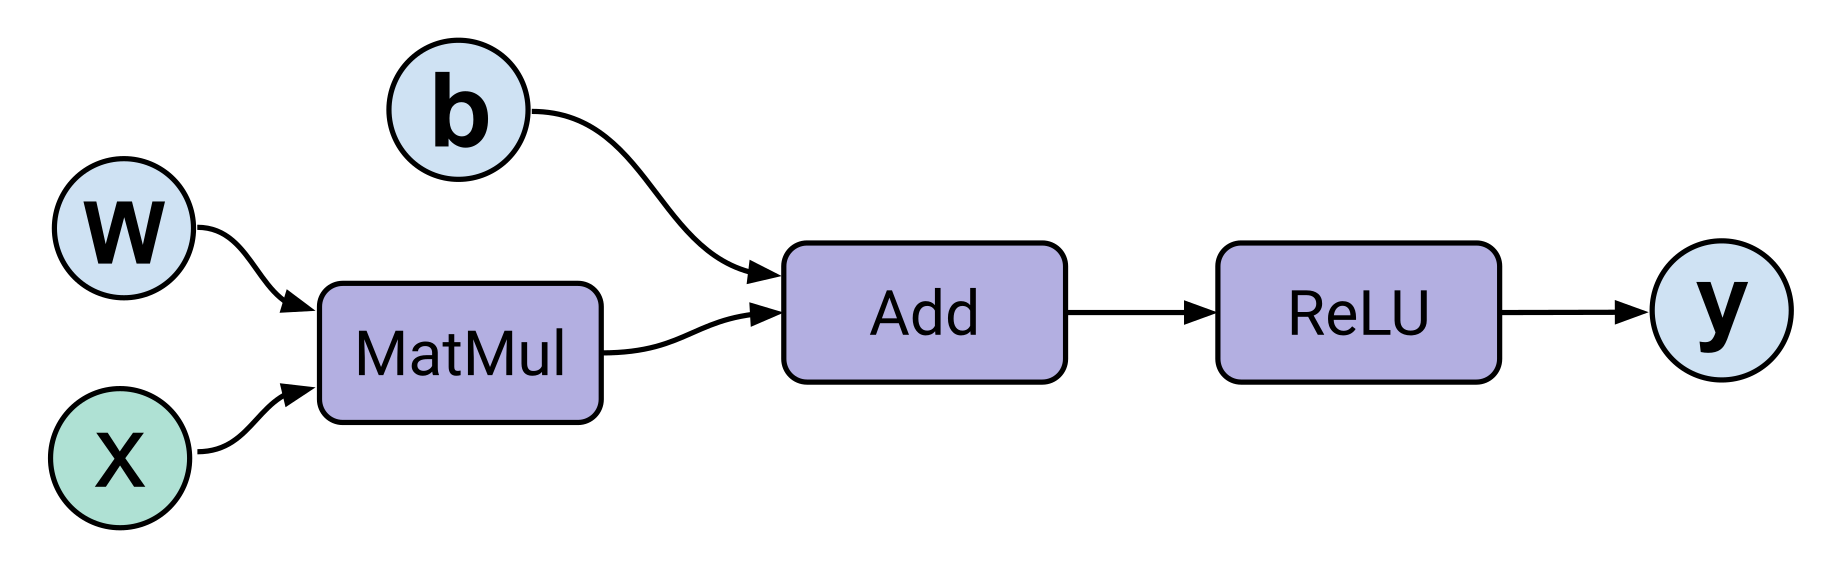
\includegraphics[width=0.75\columnwidth]{sections/2background/images/dataflow}
  \caption[Single perceptron as a computation graph]{The operations shown in purple are the nodes of the computation graph which take an arbitrary number of inputs, performs a computation at the node and produces an output. The blue nodes represent the input nodes for tensors. The directed edges show the flow of tensors through the graph.}
  \label{fig:bg:perceptron}
\end{figure}

Similarly, the whole model can be converted into a stateful dataflow (computation) graph in this manner. Using a computation graph as an intermediate representation it provides two key benefits compared to using a raw model definition. First, we can execute the model on any hardware device as the models have a single, uniform representation that can be modified as required. Secondly, it allows for pre-execution optimisations based on the host device, for example, we may perform different optimisations for executing on a GPU compared to a TPU requires different data layouts and optimisations.

\subsection{Current approaches to optimising deep learning models}
\label{sec:bg:subsec:currentapp}

Due to the prevalence and importance of machine learning, especially deep networks, there is a focus on finding ways decrease the inference runtime and by extension, increasing the model throughput. All major frameworks such as TensorFlow \cite{tensorflow2015-whitepaper}, PyTorch \cite{pytorch}, MXNet \cite{chen2015mxnet}, and Caffe \cite{jia2014caffe} have some level of support for performing pre-execution optimisations. However, the process of performing such optimisations is often time-consuming and cannot be completed in real-time. Rather, it is common to use a deep learning optimisation library such as cuDNN \cite{chetlur2014cudnn} or cuBLAS \cite{cublas2008} that instead directly optimise individual tensor operations.

%common machine learning framework is designed to greedily apply a set of pre-defined substitutions to an input graph in an attempt to optimise the graph. TensorFlow made use of low-level libraries such as cuBLAS \cite{cublas2008} for optimised matrix operations and cuDNN \cite{chetlur2014cudnn} for convolutional kernels.

%TensorRT \cite{tensorrt2017} provides a high-performance SDK to optimise the inference of models via a combination of techniques such as layout and tensor fusion, auto-tuning kernels, and multi-stream execution. The SDK acts as both the optimisation and execution engine that lies between the ML framework and physical hardware. Importantly, it is not involved during the training process, rather, it assumes for the best possible performance that the developer 

Alternatively, TVM \cite{chen2018tvm} and TensorRT \cite{tensorrt2017} can be used to optimise deep learning models and offer greater performance gains compared to the more commonly used frameworks such as TensorFlow and PyTorch. They also use greedy rule-based optimisation approaches. TODO - either expand or remove

Rather than using a rule-based optimisation approach, it is possible to use more sophisticated algorithms to optimise deep learning models at the expense of computation time. Jia et al. used a cost-based backtracking search to iteratively search through the state space of possible graphs that are provably equivalent \cite{jia2019taso}. As opposed to using rule-based optimisation that applied hand-crafted optimisations, TASO generates the candidate subgraphs automatically and formally proves the transformations are equivalent using an automated theorem prover. Furthermore, Jia et al. showed that by jointly optimising both the data layout of the subgraph transformation, and the transformation itself, TASO achieves a speedup compared to performing the operations sequentially.

A key benefit of using a cost-based approach is that the search can take into account far more complex interactions between the transformed kernels. For example, if we apply a series of transformations $T_1, \cdots, T_i$, the runtime may increase, and, due to the first set of transformations, we can now apply $T_{i + 1}, \cdots, T_{j}$, after all transformations have been applied, it is possible that we see an overall decrease in runtime. By increasing the search space of transformations in this way, Jia et al. showed that it is possible to increase the runtime of deep learning models by up to 3x \cite{jia2019taso, jia2019optimizing} compared to baseline measurements using various deep learning compilers \cite{ chetlur2014cudnn, cublas2008, tensorrt2017}.


\section{Reinforcement Learning}
Reinforcement learning (RL) is a sub-field in machine learning, broadly, it aims to compute a control policy such that an agent can maximise its cumulative reward from the environment. It has powerful applications in environments where a model that describes the semantics of the system are not available and the agent must itself discover the optimal strategy via a reward signal.

Formally, RL is a class of learning problem that can be framed as a Markov decision processes (MDP) when the MDP that describes the system is not known \cite{bellman1957}; they are represented as a 5-tuple $\langle \mathcal{S}, \mathcal{A}, \mathcal{P}_a, \mathcal{R}_a, \rho_0 \rangle$ where:

\begin{itemize}
  \item $\mathcal{S}$, is a finite set of valid states
  \item $\mathcal{A}$, is a finite set of valid actions
  \item $\mathcal{P}_a$, is the transition probability function that an action $a$ in state $s_t$ leads to a state $s'_{t+1}$
  \item $\mathcal{R}_a$, is the reward function, it returns the reward from the environment after taking an action $a$ between state $s_t$ and $s'_{t+1}$
  \item $\rho_0$, is the starting state distribution
\end{itemize}

% TODO: add citations
We aim to compute a policy, denoted by $\pi$, that when given a state $s \in \mathcal{S}$, returns an action $a \in \mathcal{A}$ with the optimisation objective being to find a control policy $\pi^*$ that maximises the \textit{expected reward} from the environment defined by \ref{equ:expec-rew}. Importantly, we can control the `far-sightedness' of the policy by tuning the discount factor $\gamma \in [0, 1)$. As $\gamma$ tends to 1, the policy will consider the rewards further in the future but with a lower weight as the distant expected reward may be an imperfect prediction.

\begin{equation}
  \label{equ:expec-rew}
  \pi^* = \argmax_\pi~\mathbb{E} \left[ \sum^\infty_{t=0} \gamma^t~\mathcal{R}_t \right]
\end{equation}

Classic RL problems are formulated as MDPs in which we have a finite state space, however, such methods quickly become inefficient with large state spaces that we consider with applications such as Atari and Go. Therefore, we take advantage of modern deep learning function approximators, such as neural networks, that makes learning the solutions far more efficient in practise. We have seen many successfully applications in a wide range of fields, for example, robotic control tasks \cite{openai2019solving}, datacenter power management, device placement, and, playing both perfect and imperfect information games to a super-human level. Reinforcement learning excels when applied to environments in which actions may have long-term, inter-connected dependencies that are difficult to learn or model with traditional machine learning techniques.

In the following sections we discuss the two key paradigms that exist in reinforcement learning and the current research in both areas and the application to systems tasks.

\subsection{Model-Free and Model-Based RL}

Model-free and model-based are the two main approaches to reinforcement learning, however, with recent work such as \cite{app10196685, kaiser2020modelbased, robine2021smaller}, the distinction between the two is becoming somewhat nebulous; it is possible to use a hybrid approach that aims to improve the sample efficiency of the agent by training model-free agents directly in the imagined environment.

The major branching point that distinguishes between model-free and model-based approaches is in what the agent learns during training. A model-free agent, in general, could learn a governing policy, action-value function, or, environment model. On the other hand, model-based agents commonly either learn an explicit representation of the parameterised policy $\pi_\theta$ using planning, such as AlphaZero \cite{silver2017mastering} or ExIt \cite{anthony2017thinking}. Alternatively, we can use use data augmentation methods to learn a representation of the underlying environment behaviour, and either only use fictitious model, or augment real experiences to train an agent in the domain \cite{kaiser2020modelbased, feinberg2018modelbased, freeman2019learning}.

Understandably, a relevant question is why one would prefer a model-free over model-based approach and what are the benefits of the respective methods. The primary benefit of model-based RL is that is has far greater sample efficiency, meaning, the agent requires in total, less interactions with the real environment than the model-free counterparts. If we can either provide, or learn, a model of the environment it allows the agent to plan ahead, choosing from a range of possible trajectories its actions to maximise its reward. The agent that acts in this ``\textit{imagined}'' or ``\textit{hallucinogenic}'' environment can be a simple MLP \cite{ha2018worldmodels} to a model-free agent trained using modern algorithms such as PPO, A2C or Q-learning. Further, training an agent in the world model is comparatively cheap, especially in the case of complex systems environments where a single episode an be on the order of hundreds of milliseconds.

Unfortunately, learning a model of the environment is not trivial. The most challenging problem that must be overcome is that if the model is imperfect, the agent may learn to exploit the models deficiencies, thus the agent fails to achieve a higher performance in the real environment. Further, learning an invalid world model can lead to the agent performing actions that may be invalid in an environment with state-dependent actions.

Model-based approaches have been successfully applied in various domains such as board games, video games, systems optimisation and robotics. Despite the apparent advantages of model-based RL with regards to reduced computation time, model-free reinforcement learning is by far the most popular approach and massive amounts of compute, typically by distributed training on clusters of GPUs/TPUs, is required overcome the sample inefficiency of model-free algorithms.

\subsection{World Models}
World models, first introduced by Ha and Schmidhuber \cite{ha2018worldmodels}, motivated and described an approach to model-based reinforcement learning in which we learn a model of the real environment using function approximators and train an agent using only predictions from the world model. Figure \ref{fig:bg:mb-rl} shows the design to utilise a world model as substitute for the real environment. In practise, a world model can be broken down into three main components. A visual model, $V$, that encodes the input into a latent vector $z$, a memory model, $M$ the integrates the historical state to produce a representation that can be used as planning for future actions and rewards. Finally, a controller, $C$ that uses both $V$ and $M$ to predict an action from the action set, $a \in \mathcal{A}$.

\begin{figure}[ht]
  \centering
  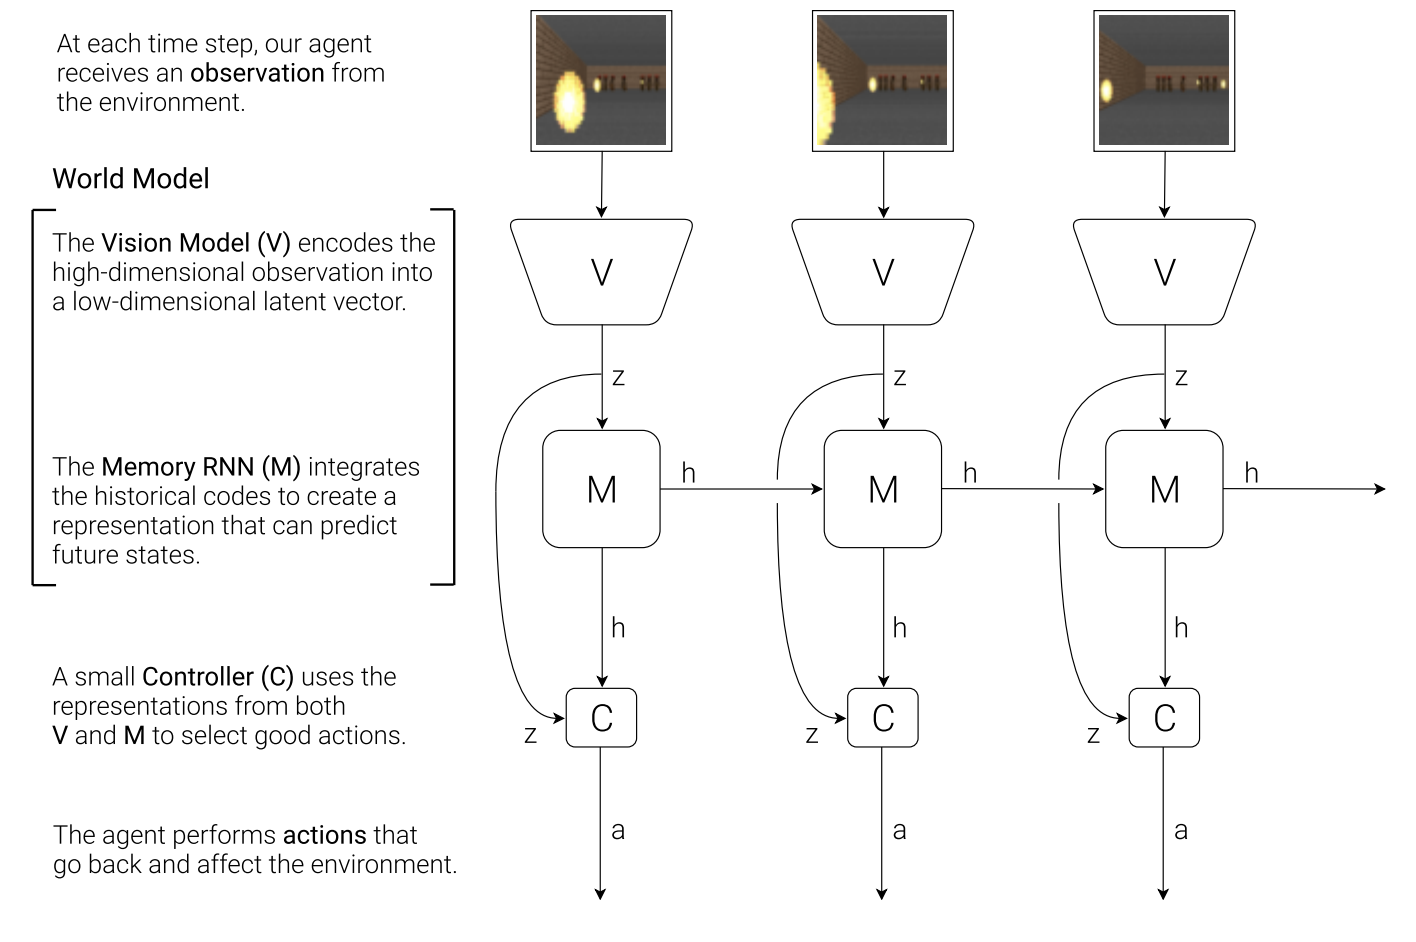
\includegraphics[width=0.75\columnwidth]{sections/2background/images/mb-rl.png}
  \caption[Model-based Reinforcement Learning End-To-End System]{Diagrammatic representation of a world-model made up from an encoder (V) that transforms the input into latent space, a `memory' module, M, that learns the behaviour of the environment from the latent vector $z$ and a controller, C, that is trained using the latent vector of the encoder and the output features from the memory to choose an action which is either applied to the real or imagined environment. Figure adapted from \cite{ha2018worldmodels}.}
  \label{fig:bg:mb-rl}
\end{figure}

Typically, a world model is trained using rollouts of the real environment that have been sampled using a random agent acting in the environment. The aim is to learn to accurately predict, given a state $s_t$, the next state $s_{t+1}$ and the associated reward $r_{t+1}$. After training, the controller, $C$, can either learn using only observations from the world model, so called ``training in a dream''. Alternatively, the world model can be used to augment the observations from the real environment samples or used only for planning. To construct the world model, if the environment is simple and deterministic, it is possible to use a deep neural network to act as the world model, however, for environments that are only partially observable, a more complex model is required such as Recurrent Neural Networks (RNNs) \cite{650093, Hochreiter:01book} or Long-short term memory (LSTMs) \cite{hochreiter1997long, gers1999learning}. The following two sub-sections describe the fundamental concepts required to construct a world model.

\subsubsection{Mixture Density Networks}
Mixture Density Networks (MDNs) are a class of neural networks first described by Christopher Bishop \cite{bishop1994mixture} that were designed to deal with problems where there is an inherent uncertainty in the predictions. Given an input to the network, we wish to output a range of possible outputs conditioned on the input where we can assess the probability of each outcome. MDNs are commonly parameterised by a neural network that is trained using supervised learning and outputs the parameters for multiple mixture of Gaussians.

\subsubsection{Recurrent Neural Networks}
Recurrent Neural Networks are class of neural networks that allows for previous outputs to be re-used as inputs to sequential nodes while maintaining and updating their own hidden state. Primarily, RNNs are commonly used in the field of speech recognition and natural language processing as they can process inputs of an arbitrary length with a constant model size. In practise however, RNNs suffer from being unable to utilise long chains of information due to the vanishing/exploding gradient problem; the gradient can change exponentially changing in proportion to the number of layers in the network \cite{Hochreiter:01book}.

Motivated by the desire to overcome the limitations of RNNs, Hochreiter et al. \cite{hochreiter1997long} developed long-short term memory by describing Constant Error Carousel (CECs). The idea was further improved by Gers et al. \cite{gers1999learning} with the modern LSTM that is made up of four gates, each with a specific purpose that influences the behaviour of each cell and in combination, the properties of the network as a whole. Figure \ref{fig:bg:lstm} shows the internal structure of an LSTM module.

\begin{figure}[ht]
  \centering
  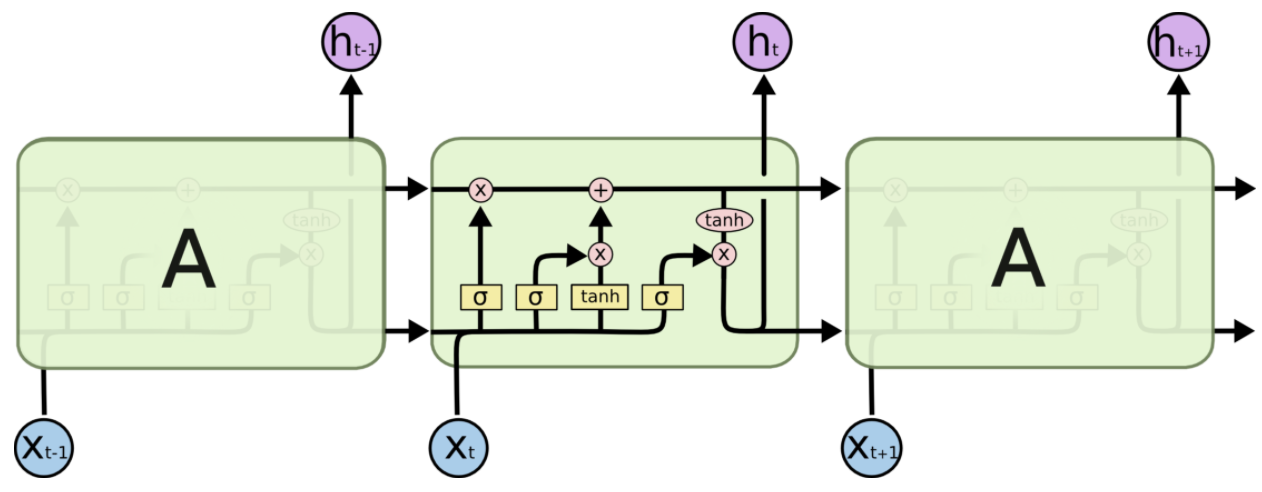
\includegraphics[width=0.75\columnwidth]{sections/2background/images/lstm.png}
  \caption[Structure of an unrolled LSTM]{LSTM}
  \label{fig:bg:lstm}
\end{figure}

An LSTM can be described using four ``gates'', where a gate influences a specific property of the LSTM cell; the four gates are as follows. The \textit{forget} gate dictates if the information stored in the cell should be erased after observing the inputs $[h_{t-1}, x_t]$; the forget gate outputs a value in the range $[0, 1]$ using the sigmoid function $\sigma$. When the forget gate output is $1$, it means to completely forget the state. Secondly, the \textit{input} gate calculates the new information to be stored in the cell; it generates a vector of candidate values defined by $\tilde{C}_t$. The \textit{update} gate is used to determine how much of the prior state sequence should be considered using the outputs from the \textit{forget} gate, the prior state $C_{t-1}$ and the input gate $\tilde{C}_t$. Finally, the \textit{output} gate determines the LSTM cell output which is based on the current, filtered state of the cell as a combination of the prior gates' output.

\begin{center}
  \begin{align*}
    f_t &= \sigma (W_f \cdot [h_{t-1}, x_t] + b_f) && (1)~\text{Forget gate} \\
    i_t &= \sigma (W_i \cdot [h_{t-1}, x_t] + b_i) && (2)~\text{Input gate} \\
    \tilde{C}_t &= \tanh (W_C) \cdot [h_{t-1}, x_t] + b_C) && (3)~\text{Candidate value} \\
    C_t &= f_t C_{t-1} + i_t \tilde{C}_t && (4)~\text{Update previous cell state} \\
    o_t &= \sigma (W_o [h_{t-1}, x_t] + b_o) && (5)~\text{Output gate} \\
    h_t &= o_t \cdot \tanh (C_t) && (6)~\text{Hidden state}
  \end{align*}
\end{center}

There are a number of popular variants of LSTM cells such as peephole LSTMs, GRUs, Grid LSTMs and ConvLSTM. There are many areas which have been revolutionised by the usage of LSTM cells in the network architecture. As we will describe in chapter \ref{sec:rlopt:subsec:rnn}, LSTM cells are the key which allows world models to learn to simulate the behaviour of the environment via state-action transitions.

\section{Graph Neural Networks}

Graph neural network are a class of neural network that has seen considerable focus in recent years, with many successful applications being devised around the central idea of leveraging the structure of the graph input to aid in predicting attributes about the graph itself. The motivation factor for the use of graph networks is that, similar to the way in which convolutional neural networks revolutionised the application of neural networks to high dimensional inputs with images, video and audio---we desire an efficient way to generalise a similar idea onto graphs to take advantage of the inductive biases.

It is often difficult to model real-world problems in a way which we can train models to take advantage of the underlying structure. Much of the data generated by real-world systems and dynamics can be modelled easily in graph form; social networks, molecules, proteins, physical systems and text all exhibit a graph structure that can be leveraged. We point the reader to the survey performed by Zhou et al. \cite{zhou2020graph} for an excellent overview of the methods and applications of graph neural networks.

Battaglia et al. \cite{battaglia2018relational} define a generalisable framework for entity/relation based reasoning with three main operators that act on edges, nodes, and on global features using user-defined functions. Within the framework described by Battaglia et al. \cite{battaglia2018relational}, a graph is defined as $G = (u, V, E)$ where $u$ are the global attributes, $V = \lbrace \mathbf{v}_i \rbrace_{i={1:N^v}}$ is the set of vertices (with a cardinality of $N^v$) and finally, $E = {(\mathbf{e}_k, r_k, s_k)}_{k={1:N^e}}$ is the set of edges with their sources and corresponding vertices.

{\SetAlgoNoLine
\begin{algorithm}[H]
 \setstretch{1.0}
 \For{$k \in \lbrace1\dots N^e \rbrace$}{
   $\mathbf{e}'_k \leftarrow \phi^e (\mathbf{e}_k, \mathbf{v}_{r_k}, \mathbf{v}_{s_k}, \mathbf{u})$
 }

 \For{$i \in \lbrace1\dots N^n \rbrace$}{
   \textbf{let} $E'_i = \lbrace (\mathbf{e}'_k, r_k, s_k) \rbrace_{r_k=i, k=1:N^e}$ \\
   $\bar{\mathbf{e}}'_i \leftarrow \rho^{e\rightarrow v} (E'_i)$ \\
   $\bar{\mathbf{v}}'_i \leftarrow \phi^{v} (\bar{\mathbf{e}}'_i, \mathbf{v}_i, \mathbf{u})$
 }

 \textbf{let} $V' = {\mathbf{v'}_{i=1:N^v}}$\\
 \textbf{let} $E' = {(\mathbf{e}'_k, r_k, s_k)}_{k=1:n^e}$\\

 $\bar{\mathbf{e}}' \leftarrow \rho^{e\rightarrow u} (E')$ \\

 $\bar{\mathbf{v}}' \leftarrow \rho^{v\rightarrow u} (V')$ \\

 $\bar{\mathbf{u}}' \leftarrow \phi^{u} (\bar{\mathbf{e}}', \bar{\mathbf{v}}', \mathbf{u})$ \\

 \Return{$(E', V', \mathbf{u}')$}

 \caption{Computation in a full GN block. Adapted from \cite{battaglia2018relational}}
 \label{algo2}
\end{algorithm}}

We can define three update functions and three \textit{aggregation} function. The update functions are $\phi^e$, $\phi^v$ and $\phi^u$ for edges, vertices and globals respectively. The aggregation functions are $\rho^{e \rightarrow v} (E'_i)$, $\rho^{e \rightarrow u} (E')$, and $\rho^{v \rightarrow u} (V')$, for edges, vertices and globals respectively. To perform a single update given a set of input edges and vertices, we simply apply the three update and aggregation functions sequentially in the order of edges, vertices, then globals. Algorithm \ref{algo:gnn} describes, in general, the algorithm to perform an update of a graph block.

% - Graph Auto-encoders

% An inductive bias is a set of assumptions that allows for the algorithm to prioritise one solution over another, while being independent from the previously observed data. 

\section{Related Work}

\textbf{Rule-based optimisation of computation graphs} is the strategy by which we transform an input graph to alter its performance characteristics. Rule-based approaches such as TensorFlow \cite{tensorflow2015-whitepaper} and TVM \cite{chen2018tvm} used a pre-defined set of transformations that are applied greedily. We evaluated our approach against these traditional approaches in section [todo: ref + extend]. In addition, recent work, such as \cite{jia2019optimizing,jia2019taso} automatically search for transformations to apply to the input graph with the modification that we allow performance decreasing transformations. Their work is similar to our approach, as we use the same automated method to discover and verify the operator transformations in an offline manner---prior to optimisation of the models. We also compare our work to TASO \cite{jia2019taso} as it is most similar in terms of substitution discovery and we present the results in section [todo].

%Rule-based approaches use a set of manually defined transformations that are applied to the input computation graph based on a set of heuristics. These methods are currently used in popular deep learning frameworks such as TensorFlow \cite{tensorflow2015-whitepaper} and compilers such as TVM \cite{chen2018tvm} to optimise the models prior to execution. In addition, recent work, such as \cite{jia2019optimizing,jia2019taso} allow the application of performance decreasing transformations in search of the most optimal graph. Furthermore, Paliwal et al. \cite{paliwal2020reinforced} used deep RL genetic algorithm to reduce runtime memory usage by optimising the placement and schedule of large models. 

% \textbf{Compilers for computation graphs}

\textbf{Model-based Reinforcement Learning} is a class of reinforcement learning algorithms in which we aim to learn---or use a given model---of the real environment in which an agent acts. The work in \cite{ha2018worldmodels} proposed a novel approach to learn a ``world model'' using recurrent neural networks; we take inspiration from such work and use world models and a policy optimisation algorithm as the controller in the world model. In contrast, alternative approaches have been proposed such as imagination-augmented agents \cite{weber2018imaginationaugmented} and model-based value estimation for model-free agents \cite{feinberg2018modelbased}. Furthermore, Nagabandi et al. \cite{nagabandi2017neural} proposed an approach to combine the sample efficiency of model-based RL and the high-task performance of model-free agents; our work differs as we use a world model to RNN-based network to simulate the environment dynamics. Other work such as \cite{robine2021smaller, hafner2021mastering} build discrete world models and train directly in latent space. Prior work on world models used a variation on a variational auto-encoders \cite{ha2018worldmodels,hafner2020dream} to generate a latent state of the pixel input, instead we use a graph neural network \cite{battaglia2018relational} to generate a latent representation of the input computation graphs.

\textbf{RL in Computer Systems} is a relatively recent topic of research. In recent years there has been an increased focused on using model-free RL in variety of systems environments. For example, in \cite{mirhoseini2017device, mirhoseini2018hierarchical, addanki2019placeto, paliwal2020reinforced}, reinforcement learning was used to optimise the placement of machine learning models to improve throughput. In \cite{app10196685}, model-based RL was used successfully to optimise the selection of bitrate when streaming data across a network. This work takes inspiration from prior work and we use both model-free and model-based RL to optimise deep learning models by reducing estimated, on-device runtime.

\textbf{Remarks.} This work distinguishes itself from the aforementioned works as, to the best of our knowledge, there has not been an attempt to use reinforcement learning, neither model-free nor model-based, to the task of optimising a deep learning model by applying substitutions directly to the computation graph. Although there has been work using RL to the task of device placement \cite{addanki2019placeto, paliwal2020reinforced} which also aims to reduce runtime or memory usage, our work is in a different domain.

%- TASO (optimising computation graphs)
%- XLA, REGAL (deepmind)
%- World models for systems environments

\chapter{Problem Specification}

In this chapter we will introduce the graph optimisation problem and establish the baseline performance using cost-based backtracking optimisation. Next, we will frame the optimisation problem in the RL domain by describing the system environment, the reward calculation and the state-action space. Additionally, we describe the RL agents trained in the model-free and model-based domains and we also highlight limitations in the application of reinforcement learning to this problem.

\section{Introduction}
The major deep learning frameworks such as TensorFlow \cite{tensorflow2015-whitepaper} and PyTorch \cite{pytorch} used greedy rule-based graph transformation prior to execution. Furthermore, in Chapter \ref{sec:bg:subsec:currentapp} we described the prior work upon which this work builds. Namely, we introduced the work by Jia et al. \cite{jia2019taso,jia2019optimizing} that proposed an approach for performing an offline optimisation of deep learning computation graphs using a recursive backtracking search in the action space. Specifically, the authors developed a framework that uses a pre-generated set of formally verified, semantically equivalent graph substitutions that can be used to modify the graph to search for a reduced runtime.

\section{Optimisation of deep learning graphs}

TensorFlow (TF) uses a system called \textit{``Grappler''} that is the default graph optimisation system in the TF runtime \cite{larsen2019tensorflow}. By natively performing the graph optimisation at runtime, it allows for a interoperable, transparent optimisation strategy via protocol buffers. To improve the performance of the underlying model, Grappler supports a range of features such as the pruning of dead nodes, removal of redundant computation and improved memory layouts. Concretely, Grappler was designed with three primary goals:

\begin{itemize}
  \item Automatically improve performance through graph simplifications and high-level optimisations to benefit the most target architectures
  \item Reduce device peak memory usage
  \item Improve hardware utilisation by optimising device placement
\end{itemize}

On the other hand, although Grappler can automatically optimise the data-flow graphs of deep learning models, such a complex optimisation system presents challenges. Firstly, significant engineering effort is required to implement, verify and test the optimiser to ensure the correctness of the graph rewrites rules; TF contains a set of 155 substitutions that are implemented in 53,000 lines of code; to further complicate matters, new operators are continuously proposed, such as grouped or transposed convolutions, all of which leads to a large amount effort expended to maintain the library. Secondly, and perhaps more importantly, as TF uses Grappler at runtime by default, it adds overhead to execution as extra graph conversions are performed at runtime rather than offline.

\begin{figure}[ht]
  \centering
  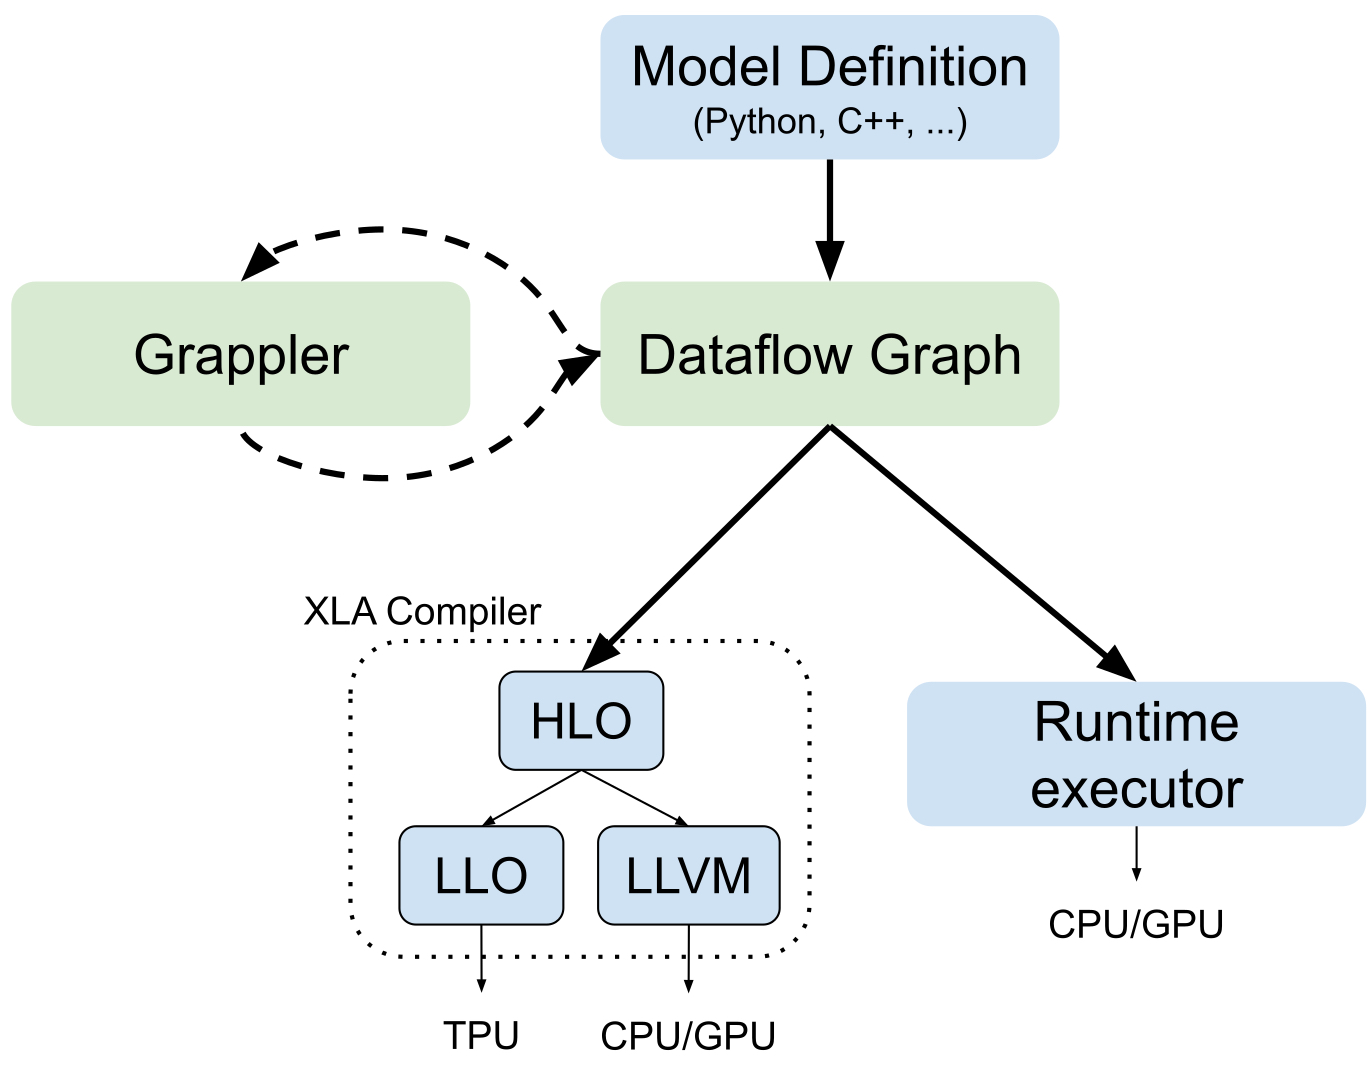
\includegraphics[width=0.75\columnwidth]{sections/3problem/images/GraphOptimiser.jpg}
  \caption[Architecture of graph optimisation system in TensorFlow]{The machine learning model is processed prior to execution by either Grappler, the static graph optimiser in TensorFlow, or via JIT compilation of the model using XLA. Figure adapted from \cite{larsen2019tensorflow}.}
  \label{fig:problem:graph-optim}
\end{figure}

Alternatively, both TensorFlow, and more recently PyTorch, support automatic graph optimisation by JIT (just-in-time) compilation through XLA and the \texttt{torch.jit} package respectively. In Figure \ref{fig:problem:graph-optim} we can see a high-level view of the components of the optimisation system. In order to motivate the reasoning to perform offline optimisation rather than JIT optimisation we  consider the work proposed by Jia et al. in both MetaFlow and TASO, the systems they design can be used as a drop-in replacement of the Grappler and/or XLA compilation steps.

TASO applies all possible candidate transformations at each step and estimates the runtime (or cost) of the final graph. Next, TASO chooses the highest performing candidates for the proceeding iteration of candidate evaluations. Principally, this approach is superior to the naive greedy optimisation approach as we can use the estimated runtime to guide the search and forego immediate improved runtime to increase the potential search space of candidate graphs.

In addition, as TASO operates at the graph-level, its optimisations are completely orthogonal to operator-level optimisations; thus it can be combined with code generation techniques such as TVM \cite{chen2018tvm} or Astra \cite{sivathanu2019astra} to further improve overall performance. We also note that TASO performs tensor data layout and graph transformation simultaneously rather than sequentially. It has been shown that by considering it as a joint optimisation problem end-to-end inference runtime can be reduced by up to 1.5x \cite{jia2019taso, jia2019optimizing}.

% However, using estimated runtime presents a challenge with respect to the exponential growth of search space at a rate of $O(N^T)$, where $N$ is the number of transformations and $T$ is the number of search steps.

\subsection{Graph-level optimisation}

Performing optimisations at a higher, graph-level means that the resulting graph is - in terms of execution methodology - no different than the original graph prior to optimisation. Therefore, by performing graph-level optimisation we generate a platform and backend independent graph representation which can be further optimised by specialised software for custom hardware accelerators such as GPUs and TPUs.

Next, we define that two computation graphs, $\mathcal{G}$ and $\mathcal{G}'$ are semantically equivalent when $\forall \mathcal{I} : \mathcal{G}(\mathcal{I}) = \mathcal{G}'(\mathcal{I})$ where $\mathcal{I}$ is an arbitrary input tensor. We aim to find the optimal graph $\mathcal{G}^*$ that minimises the cost function, \texttt{cost}$(\mathcal{G})$, by performing a series of transformations to the computation graph - at each step, the specific transformation applied does not need to be strictly optimal. In fact, by applying optimisations that reduce graph runtime we further increase the state space for the search; a large state space is preferable in the reinforcement learning domain.

An important problem in graph-level optimisation is that of defining a set of varied, applicable transformations that can be used to optimise the graphs. As previously noted, prior work such as TensorFlow use a manually defined set of transformations and optimise greedily. On the other hand, TASO uses a fully automatic method to generate candidate transformations by performing a hash-based enumeration over all possible DNN operators that result in a semantically equivalent computation graph.

\begin{figure}[ht]
  % preliminary
  \sbox\twosubbox{%
    \resizebox{\dimexpr.9\textwidth-1em}{!}{%
      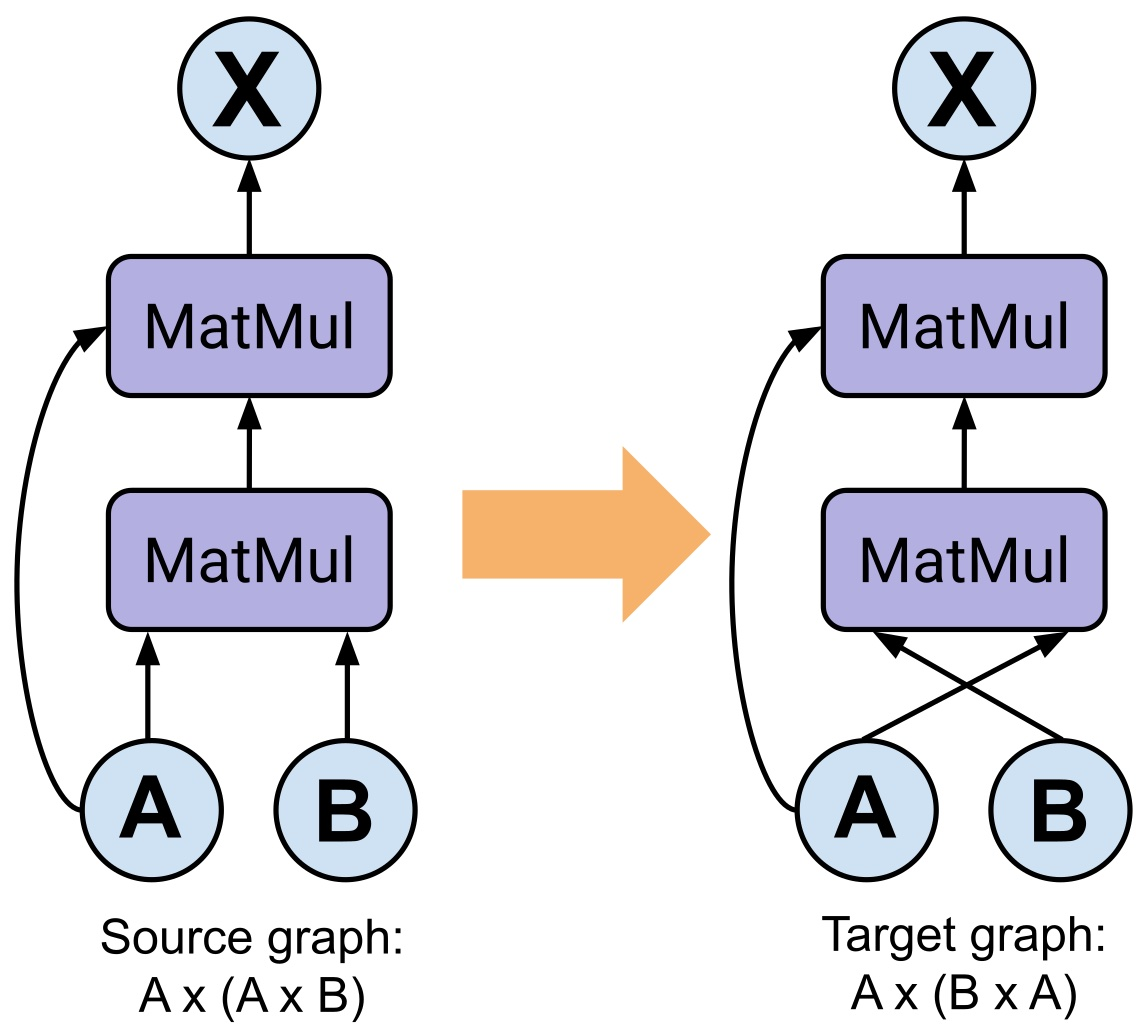
\includegraphics[height=3cm]{sections/3problem/images/rewrite1.jpg}%
      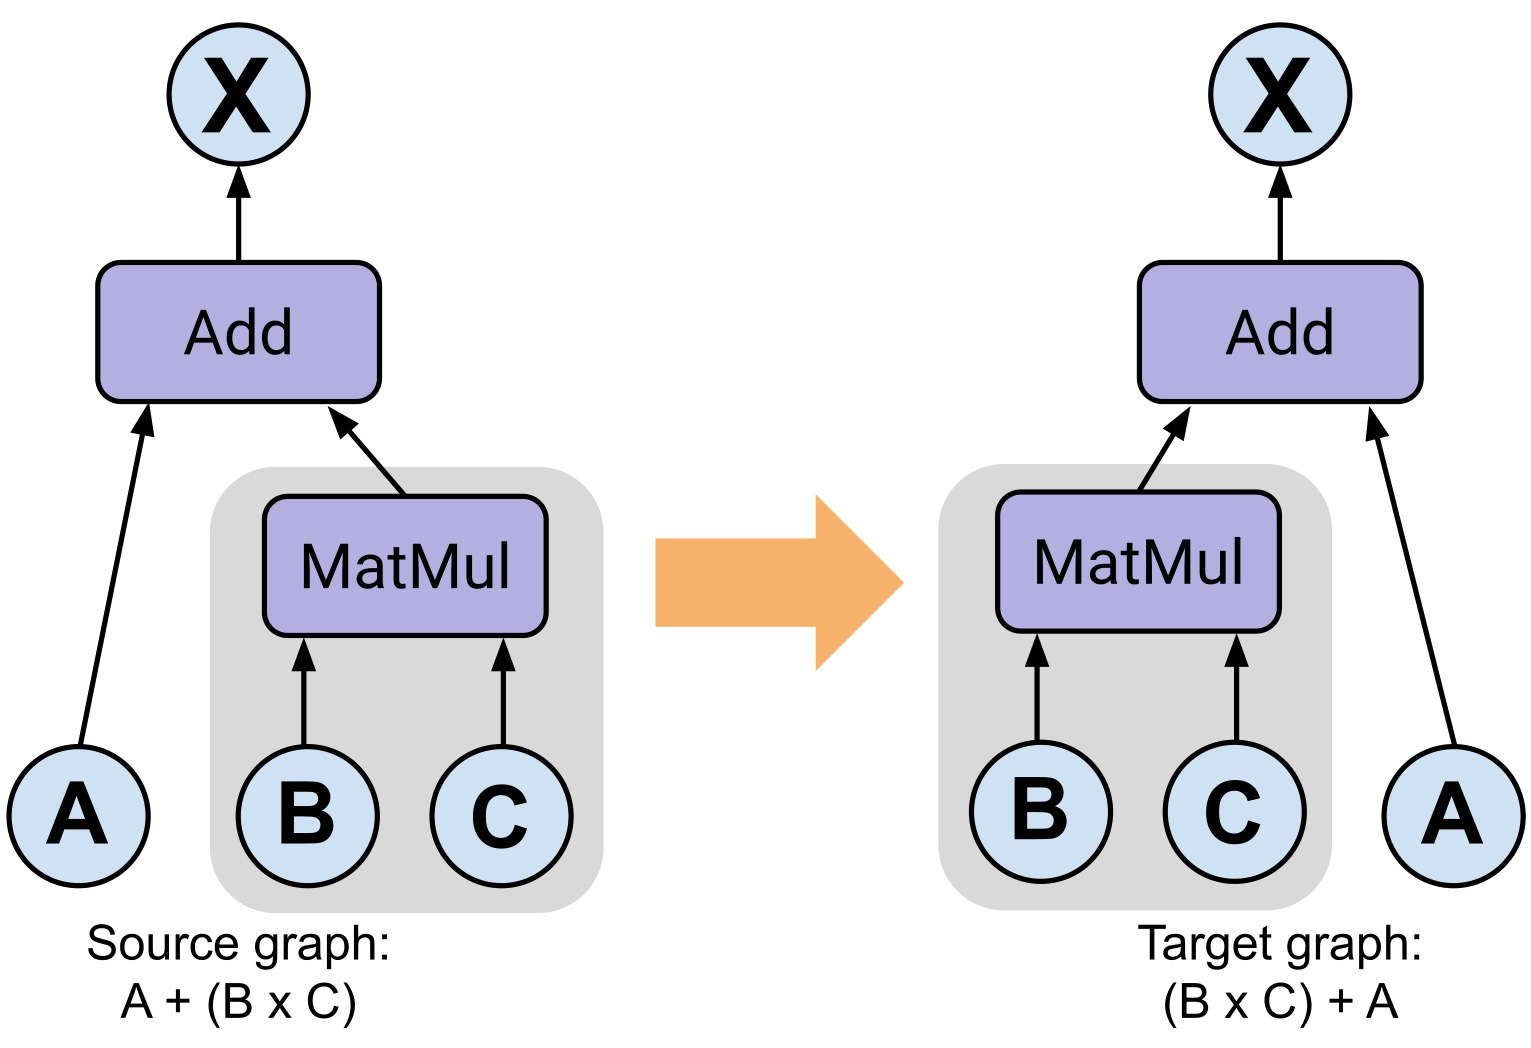
\includegraphics[height=3cm]{sections/3problem/images/rewrite2.jpg}%
    }%
  }
  \setlength{\twosubht}{\ht\twosubbox}
  
  % typeset
  \centering
  \subcaptionbox{Tensor renaming substitution \label{fig:problem:rewrite-graph1}}{
    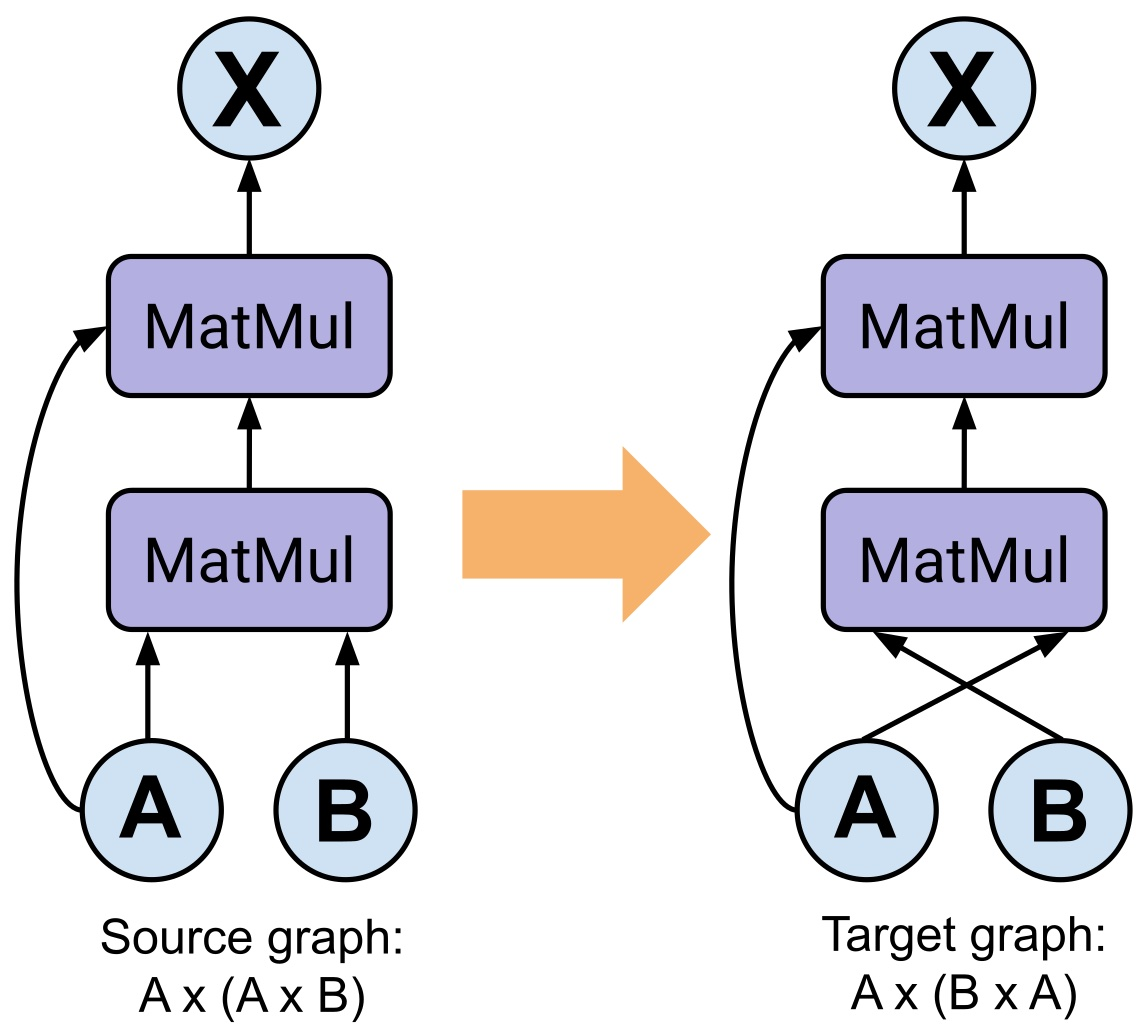
\includegraphics[height=\twosubht]{sections/3problem/images/rewrite1.jpg}
  }\quad
  \subcaptionbox{Common subgraph substitution \label{fig:problem:rewrite-graph2}}{
    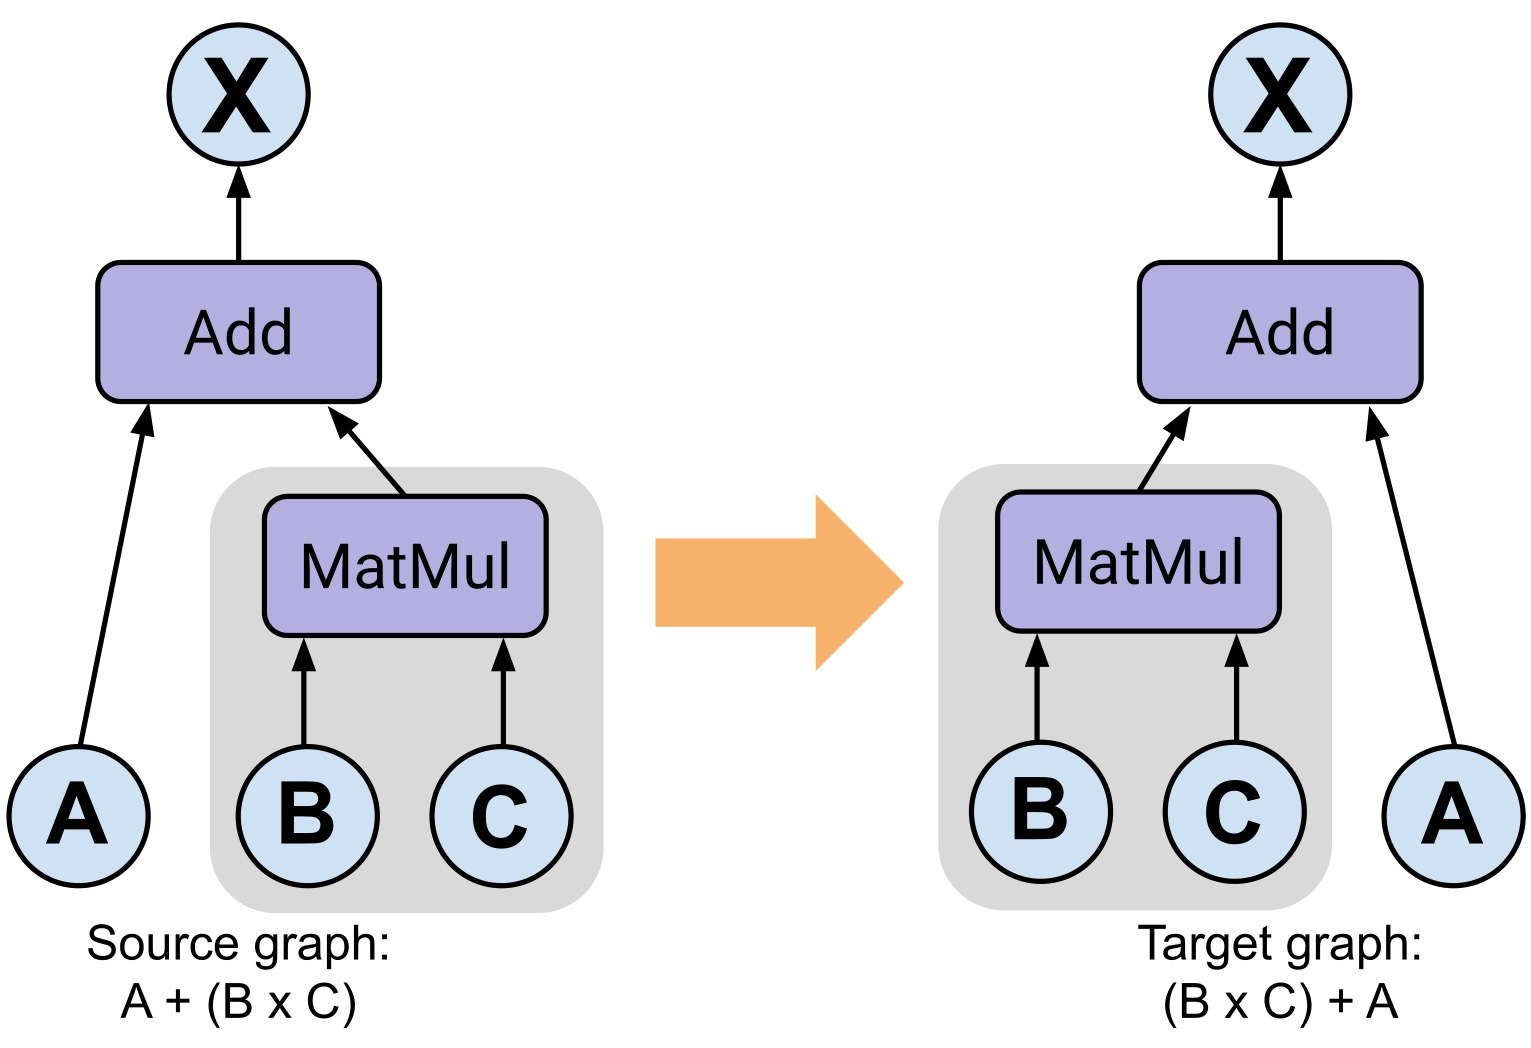
\includegraphics[height=\twosubht]{sections/3problem/images/rewrite2.jpg}
  }
  \caption[Two examples of trivial graph substitutions]{Two examples of trivial graph substitutions that does not impact the overall runtime of the computation graph. The left sub-figure shows a simple renaming of the tensor inputs. The figure on the right shows that we have a common sub-graph between the source and the target graphs. In both cases we eliminate the duplicates as the hash of the two graphs will be identical.}
\end{figure}

In this work, we take the same approach as that of TASO and automatically generate the candidate graphs. We perform this as an offline step as it requires a large amount of computation to both generate and verify the candidate substitution; to place an upper bound on the computation, we limit the input tensor size to a maximum of 4x4x4x4 during the verification process. Following the generation and verification steps, we prune the collection to remove substitutions that are considered trivial and as such would not impact runtime. For example, trivial substitutions include input tensor renaming and common subgraphs, we show both techniques diagrammatically in Figure \ref{fig:problem:rewrite-graph1} and \ref{fig:problem:rewrite-graph2} respectively.

- TODO: TASO algo for searching for optimal graph

\subsection{Baselines}
In order to establish a baseline performance measure for performing graph-level optimisation of deep learning models we have two different sources. Firstly, we can measure the performance of a select number of deep learning models in the standard DL frameworks, TensorFlow and PyTorch. In this project, there are common, standardised mechanisms for evaluating the performance of models using these frameworks - we show the results of the baseline measurements in the following section.

Secondly, in this work, we replicate the experiments as performed by Jia et al. \cite{jia2019taso} and use the results as our benchmark to compare our work against. However, for the majority of evaluated graphs we used a lower budget than that of the authors in the original paper. We found that using a lower search budget, without alteration of the hyperparameter $\alpha$, it did not result in a lower performance compared to the original experiments. Figure [TODO] shows the results of the heuristic search for the graph $\mathcal{G}^*$ and Figure [TODO] shows the relative performance of the methods on each chosen deep learning model. 

% {\SetAlgoNoLine
\begin{algorithm}[H]
 \setstretch{1.0}
 \textbf{Input}: Initial computation graph $\mathcal{G}_0$, a cost function \texttt{cost}($\mathcal{G}$), a list of valid graph substitutions $\lbrace S_1, \dots, S_m$, and the hyperparameter $\alpha$ \\

 \textbf{Output}: An optimised computation graph $\mathcal{G}^*$

 \texttt{//} $\mathcal{Q}$ is a priority queue of graphs sorted under \texttt{cost}.\\
 $\mathcal{Q} = \lbrace \mathcal{G}_0 \rbrace$

 \While{$\mathcal{Q} \neq \lbrace \rbrace$}{
   $\mathcal{G} = \mathcal{Q}$.\texttt{dequeue()}\\
   \For{$i = 1 \dots m$}{
    $\mathcal{G}' = S_i(\mathcal{G})$ \\
    \If{\texttt{cost}($\mathcal{G}'$) $<$ \texttt{cost}($\mathcal{G}^*$)}{
      $\mathcal{G}^* = \mathcal{G}'$
    }
    \If{\texttt{cost}($\mathcal{G}'$) $< \alpha~\times$ \texttt{cost}($\mathcal{G}^*$)}{
      $\mathcal{Q}$.\texttt{enqueue($\mathcal{G}'$)}
    }
  }
 }
 \Return{$\mathcal{G}^*$}

 \caption{Cost-based backtracking search. Adapted from \cite{jia2019taso}.}
 \label{algo3}
\end{algorithm}}

% - Estimation of runtime characteristics for each tensor op --> imperfect estimation

% - Using real runtime is difficult as it takes longer to simulate and large variation in measurements between runs

\section{Reinforcement Learning formulation}
In the following section we will describe how to represent the computation graph optimisation problem in the reinforcement learning domain by describing the key components of the system. We describe the system environment in which the agents act, the state-action space, and finally the reward functions for both the model-free and model-based agents which we used to determine the optimal reward signal to train the agents.

\subsection{System environment}

In order to train a reinforcement learning agent, it necessary that we have access to an environment that, given the current environment state, the agent can take an action. After taking the chosen action, the environment is updated into a new state and the agent receives a reward signal. Typically, one uses a mature environment such as OpenAI Gym \cite{brockman2016openai} or OpenSpiel \cite{LanctotEtAl2019OpenSpiel} as the quality of the environment often has a significant effect on the stability of training. Moreover, using an environment that uses a common interface allows researchers to implement algorithms with ease and, importantly, reproduce results from published conference papers.

In our work, we implemented an environment that follows the OpenAI Gym API standard stepping an environment, that is, we have a function \texttt{step(action)} that accepts a single parameter, the action requested by the agent to be performed in the environment. The \texttt{step} function returns a 4-tuple \texttt{(next\textunderscore state, reward, terminal, extra\textunderscore info)}. \texttt{extra\textunderscore info} is a dictionary which can store arbitrary data. The environment in our project has a structure that is shown diagrammatically in Figure [TODO].

To simplify the implementation of the environment, we used made extensive use of the work by Jia et al. \cite{jia2019taso} with the open source version of TASO. We provide a computation graph and the chosen transformation and location; TASO then applies the requested transformation and returns the newly transformed graph. Further, we use internal TASO functions that calculates estimates of the runtime on the hardware device which we use as our reward signal for training the agent. During our experiments we modified TASO to extract detailed runtime measurements to analyse the rewards using a range of different reward formulae - we describe our approach further in section \ref{sec:prob:subsec:rwd}.

The scope of our work meant that there was no existing prior work that applied reinforcement learning to the task of optimising deep learning computation graphs. Thus, we required an environment in which an agent can act efficiently. Due to the nature of systems environments, the interactions with the real-world environment can be often slow, especially compared to those such as Arcade Learning Environment \cite{Bellemare_2013}. An aim of this work was to train a simulated environment, a ``world model'', that if accurate in relation to the real environment, we can train an agent far more efficiently than would be possible with the real-environment. In section [TODO] we will further explore world models and evaluate our implementation.

\subsection{State-Action space}
In this project we modelled the state and action space in accordance with prior research, specifically we referenced work in a similar domain of system optimisation using reinforcement learning; Mirhoseini et al. \cite{mirhoseini2018hierarchical} used hierarchical RL with multiple actions to find the optimal device placement and Addanki et al. \cite{addanki2019placeto} that also aided in the design choice of input/output graph sizes.

The environment expects two actions: 
\begin{itemize}
  \item Transformation (which we refer to as an \texttt{xfer}) to apply, \texttt{xfer\textunderscore ID}
  \item Location at which to apply the transformation
\end{itemize}
Therefore, we define the action as 2-value tuple of (xfer\textunderscore, location). There is a special case for the xfer\textunderscore id. If this is N (i.e. 151), this is the no-op action. This will not apply any XFER to the graph, but instead end the current episode (the done value will be True and depending on the reward mechanism, the reward will be calculated).

As explained in the previous section, we used an step-wise approach where at each iteration, we provide a 2-tuple of the transformation and location, to apply in the current state. The updated state from the environment is a 4-tuple consisting of \texttt{(graph\textunderscore tuple, xfer\textunderscore tuples, location\textunderscore masks, xfer\textunderscore mask)}.

\texttt{xfer\textunderscore mask} refers to a binary mask that indicates the valid and invalid transformations that can be applied to the current computation graph as not every transformation can be applied to every graph. If the current graph has only four possible transformations that can be applied, all other transformations considered to be invalid. Thus, we return a boolean location mask where only valid transformations are set to 1, or \texttt{true}. This can be used to zero-out the model logits of invalid transformations (and thereby actions also) to make ensure the agent always selects a valid transformation from the set.

Similarly, for each transformation selected by the agent, there are a number of valid locations where this transformation can be applied. We set a hardcoded, albeit configurable, limit the number of locations to 200 in this work. If the current graph has fewer than 100 possible for any given transformation, the remaining locations are considered invalid locations. Therefore, we again return a boolean location mask, which is named \texttt{location\textunderscore masks} in the 4-tuple defined above, which can be used to zero out the model logits of invalid locations.

% We do this for every XFER, so this is a N x L array, where N is the number of XFERs (currently 151) and L is the maximum number of valid locations (per default 100).

\subsection{Reward determination}
\label{sec:prob:subsec:rwd}
- Runtime difference

- Inclusion of detailed measurements

- Real-time measurements instead of estimated?

- Look up research on RL rewards (what makes a good reward signal)


\chapter{Reinforcement Learning Agent Design}

\section{Model-free Agent}

In section \ref{sec:design:subsec:embed} we described the process for translating the computation graph, built in a machine learning framework, into an internal message passing graph neural network that can produce a latent space embedding, $z_t$, of the graph state $s_t$ at a time $t$. In our work, we used the PPO algorithm  described by Schulman et al. \cite{schulman2017proximal} to select actions as it brings three advantages. PPO was deliberately designed to be sample efficient, easy to implement, and stable to a wide range of values in hyperparameter selection. Its predecessors, such as TRPO \cite{schulman2017trust}, required off-policy learning using replay memory, which is often challenging to implement efficiently---especially with systems environments where rollouts are expensive to collect and store. Algorithm \ref{algo:ppo} shows a variant of the PPO algorithm using a clipped objective, resulting in a simpler implementation compared to KL-penalty objective.

% Moreover, PPO is an on-policy algorithm that is compatible with stochastic gradient descent (SDG), meaning we can use it in combination with our graph network to train using hierarchical reinforcement learning. 

% We chose to use hierarchical reinforcement learning (HRL) to structure the learning of the model-free agent by breaking down the action predictions into sub-policies. As hypothesised by Nachum et al. \cite{nachum2019does}, HRL provides a unique benefit of improved environment exploration by temporally extended exploration as high-level actions correspond to multiple environment steps, thus, the HRL agent can explore more efficiently.

{\SetAlgoNoLine
\begin{algorithm}[H]
\setstretch{1.0}
 Input: initial policy parameters $\theta_0$, clipping threshold $\epsilon$ \\
 \For{k = 0, 1, 2, \dots}{
  Collect set of partial trajectories $\mathcal{D}_k$ on policy $\pi_k = \pi(\theta_k)$ \\
  Estimate advantages $\hat{A}_t^{\pi_k}$ using GAE with the value function $V_{\phi_k}$ \\
  Compute policy update
  \[
  \theta_{k+1} = \argmax_{\theta} \mathcal{L}_{\theta_k}^{\text{CLIP}}(\theta)
  \]
  by taking $K$ steps of minibatch SDG (using Adam), where
  \[
  \mathcal{L}_{\theta_k}^{\text{CLIP}}(\theta) = \mathbb{E}_{\tau \sim \pi_k} \left[ \sum_{t=0}^T \left[ \min (r_t(\theta) \hat{A}_t^{\pi_k}, \text{clip}(r_t(\theta), 1 - \epsilon, 1 + \epsilon) \hat{A}_t^{\pi_k}) \right] \right]
  \]
 Fit value function using using MSE loss using minibatch SDG
 \[
 \phi_{k+1} = \argmin_{\phi} \frac{1}{|\mathcal{D}_k|T}  \sum_{t=0}^T \left( V_\phi \left( s_t \right) - \hat{R}_t \right)^2
 \]
 }
 \caption{PPO with Clipped Objective. Adapted from \cite{schulman2017proximal}.}
 \label{algo:ppo}
\end{algorithm}}

We use short online rollouts to collect a mini-batch of observations where a single trajectory begins with the unmodified graph and we iteratively apply transformations until we reach a terminal action or no further transformations can be applied. After each rollout we estimate the runtime which is used to calculate the reward for the rollout---we describe the reward calculation in section \ref{sec:prob:subsec:rwd}.

After collection of $n$ rollouts, we train the agent using the data produced during each action step which is used to update the weights of the policy and value neural networks according to the PPO algorithm. One should note that as we require two actions to be selected (\texttt{xfer\textunderscore id} and \texttt{location\textunderscore id}), it requires two sets of results to be collected during the rollout, one for each action performed. Additionally, as we perform two actions, it doubles our overhead during training as we both store and perform backpropagation for four neural networks, the policy and value networks for each action. However, as we discussed in \ref{sec:prob:subsec:sap}, the alternative approach we considered would lead to lower agent performance during training due to the larger action space.

\section{Model-based Agent}

Unlike model-free reinforcement learning, in the domain of model-based reinforcement learning we aim to learn a model of the environment such that we no longer need the real simulator, providing numerous benefits such as improved sample efficiency, ability to plan trajectories of actions forward in time and decreased training time for systems environments. The primary task is model-based RL is to learn a model of the environment. Concretely, we aim to learn a function $f(z_t, a_t)$ that predicts the latent next state $z_{t+1}$ based on the action $a_t$ being performed in the state $z_t$, the reward $r_t$ and the terminal flag $d_t$ which indicates the end of the trajectory. Many environments, especially systems tasks, state transitions are stochastic and we must accurately represent such transitions in order to have a useful world model for planning. This section will further discuss how we designed the world model for learning the environment behaviour.

\subsection{World Models}
World models, introduced by Ha et al. \cite{ha2018worldmodels}, create an imagined model of the true environment by observing sequences of states, actions and rewards from the environment and learning to estimate the transitions between states based upon the actions taken. Ha et al. showed that the world models can learn the environment transitions and achieve state-of-the-art results on visual learning tasks such as CarRacing and VizDoom. One should note that Ha \& Schmidhuber used  a latent space embedding from the convolutional neural network based on the RGB pixel image; in this work we instead use the latent space produced by the graph neural network - in either case, we are learning the world model using the latent space of the environment. World models are constructed from three components. The ``visual'' module, taking the raw state from the environment and transforming into latent space, as well as the ``memory''  and ``controller`` modules which are discussed below.

\subsubsection{Mixture Density Networks}
Mixture Density Networks (MDNs) are a class of network that can learn to output parameters to a probabilistic Gaussian mixture model (GMMs) \cite{bishop1994mixture}. A GMM is a function that is composed of several gaussians, each given a label $k \in \lbrace 1, \ldots, K \rbrace$, where $K$ is the number of components. Each gaussian is formed from three parameters $\mu_i$, the mean of component $i$, $\sigma_i$ the variance of component $i$ and $\pi$ the mixing probability/weight of each component. Unlike the networks used in supervised learning tasks that are trained using regression, training a GMM instead attempts to maximise the likelihood that the gaussians fit the data points in each minibatch. Inside a world model we use the predictions of an MDN at time $t$ to choose the parameters of the gaussian distribution for the next latent vector at time $t+1$. Notably, one can either use expectation maximisation to find the parameters of the model, or alternatively, can use a parameterised GMM which is trained in conjunction with the RNN using stochastic gradient descent.


\subsubsection{Recurrent Neural Networks}
Recurrent Neural networks (RNNs) are a class of architectures in which the connections between the nodes form a directed graph in a temporal sequence \cite{650093}. There are many forms which an RNN can take, each providing features and levels of stability which one many find useful for the task at hand. Importantly, the output of an RNN is deterministic, however, we can use the outputs from the RNN as the parameters for a probabilistic model to insert a controllable level of stochasticity in the output predictions \cite{graves2014generating}.

\begin{figure}[ht]
  \centering
  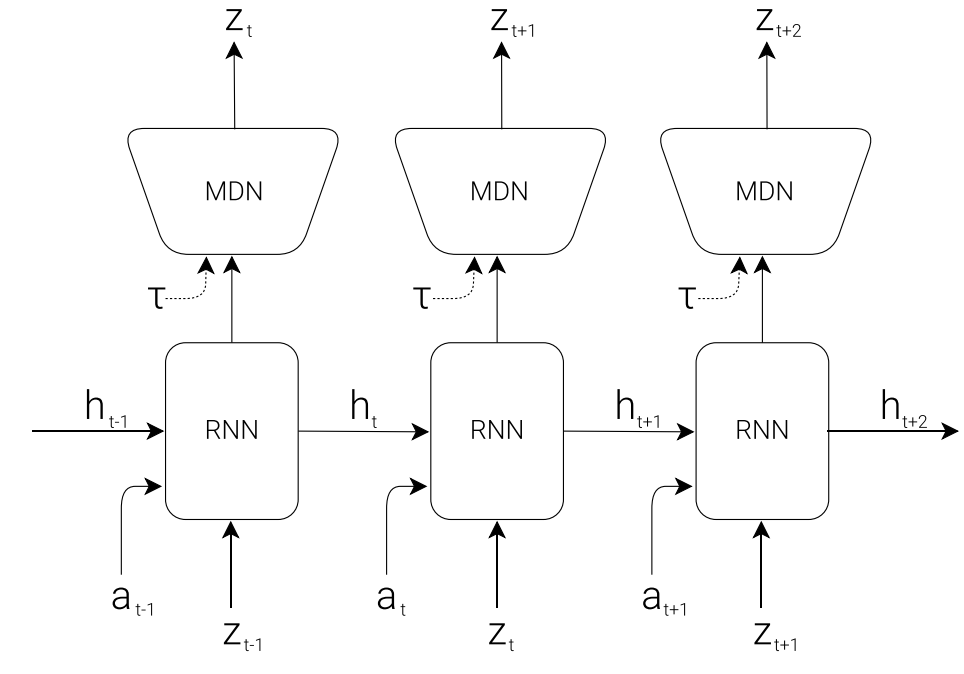
\includegraphics[width=0.75\columnwidth]{sections/4rlopt/images/mdnrnn.png}
  \caption[Temporally unrolled MDN-RNN]{Structure of an unrolled MDN-RNN. The MDN outputs the parameters of a Gaussian mixture distribution used to sample a prediction of the next latent vector $z_{t+1}$, the MDN is controlled by the temperature parameter $\tau$.}
  \label{fig:rl:mdnrnn}
\end{figure}

A constraint of using RNNs is that they expect a fixed sized input sequence. However, in our work, both the shape of the latent state tensor, and the number of actions performed by the agent in a rollout is variable. As such, we employ a common approach to mitigate this problem is by prepending zero values to the input sequence until the desired length is reached, commonly referred to as padding. After performing inference on the model and retrieving the predicted state, we mask the results based on the input padding to ensure we only use valid predictions to select the next action using the controller.

\subsubsection{MDN-RNN}

By combining the mixture density and recurrent networks, we can use rollouts of the environment sampled using a random agent to train the combined network, called an MDN-RNN. We use the network to model $P(z_{t+1}~|~a_t, z_t, h_t)$, where $z_t$, $z_{t+1}$ is the latent state at the times $t$ and $t+1$ respectively, $a_t$ is the action taken at time $t$, and $h_t$ is the hidden state from the RNN network at time $t$. Figure \ref{fig:rl:mdnrnn} shows the combination of the RNN and MDN networks and how we calculate the predictions of the next latent state in sequence.

Furthermore, after training the world model, we must train an agent (or controller) to perform actions in the world model and learn to take optimal actions that maximise reward. During inference of the world model, we use a softmax layer which outputs $\pi$ in the form of a categorial probability distribution which we sample under the Gaussian model parameterised by $(\mu_i, \sigma_i)$.

In figure \ref{fig:rl:mdnrnn} we show that one of the inputs to the MDN is $\tau$, the temperature. By altering the temperature it allows us to control the stochasticity of the agent during training of the controller. The logits of the RNN that represent the predictions for the values of $\pi$ are divided by the temperature prior to being passed into the softmax function which converts the logits into pseudo-probabilities. We incorporate the temperature, $\tau$, into the softmax function using the following equation.

$$
\text{softmax}(\mathbf{x}_i) = \frac{\exp\left( \nicefrac{x_i}{t} \right) }{\Sigma_j \exp \left( \nicefrac{x_j}{t} \right) }
$$

Typically, temperature is a real number in the range $\tau \in \left( 0, \ldots, 1 \right)$, where a value of zero leads to completely deterministic predictions generated by the RNN, whereas larger values introduces a greater amount of stochasticity in the predictions. As larger values of $\tau$ increases the probability of samples with a lower sampling likelihood being selected it leads to a greater diversity of actions taken by the agent in the environment. Importantly, Ha et al. \cite{ha2018worldmodels} found that having a large temperature can aid in preventing the agent from finding strategies to exploit inadequacies in the world model.

\subsection{Action Controller}

\chapter{Evaluation}

\section{Aims}

In this chapter, we look to assess aims we presented at the beginning of this work where we claimed to use reinforcement learning to perform automated optimisation of deep learning computation graphs. Thus, this evaluation seeks to answer the following questions:

\begin{enumerate}
  \item Are model-based reinforcement learning methods able to model the transition dynamics of the environment?
  \item Is the agent policies able to generalise to unseen states of the same graph to act in accordance to our performance objectives?
  \item Do the world models accurately model the reward estimation from the graphs latent state?
  \item Are the agents trained in an imagined world model applicable to the real-world environment?
\end{enumerate}

Throughout this chapter, we aim to answer these questions by a series of experiments which provide evidence to support our claims. Finally, we conclude with an overall discussion of our findings and its impact.

\section{Experimental Setup}

All the experiments presented in this chapter, both training various agent models and testing, is performed using the codebase available in the GitLab repository for this project \footnote{\url{https://www.gitlab.com/CamRL/xflowrl}}. The project was developed, and the experiments were performed using a single machine running Ubuntu Linux 18.04 with a 6-core Intel i7-10750H@2.6GHz, 16GB RAM and an NVIDIA GeForce RTX 2070.

To interface with the internal representation of the computation graphs, as previously discussed, we used the open-sourced version of TASO \cite{jia2019taso} which we modified to extract detailed runtime information. Further, we implemented the reinforcement learning algorithms in TensorFlow 2 \cite{tensorflow2015-whitepaper} and utilised the \texttt{graph\textunderscore nets} package developed by Battaglia et al. \cite{battaglia2018relational} to process our input graphs which we described in chapter \ref{sec:prob:subsec:sysenv}. The PPO agent was implemented based upon the implementation provided by Schulman et al. \cite{schulman2017proximal}.

\subsection{Graphs Used}
\label{sec:eval:subsec:graphsused}

\begin{table}[htbp]
  \centering
  \resizebox{\columnwidth}{!}{
    \begin{tabular}{@{}llllll@{}}
      \toprule
                    & InceptionV3   & ResNet-18     & ResNet-50     & SqueezeNet1.1 & BERT        \\ \midrule
      Type          & Convolutional & Convolutional & Convolutional & Convolutional & Transformer \\
      Layers        & 43            & 18            & 50            & 21            & 12          \\
      Unique Layers & 12            & 6             & 6             & 3             & 3           \\
      Substitutions & 56            & 40            & 228           & 288           & 80          \\ \bottomrule
      \end{tabular}
  }
  \caption[Properties of evaluation graphs]{Properties of the five evaluation graphs used in the experiments contained in this chapter. We differentiate the total number of layers in a network from the number of unique layers used in composing the network to provide a more accurate representation of its complexity.}
  \label{table:eval:graph-props}
\end{table}

We chose to use five real-world deep learning models to evaluate our project. InceptionV3 \cite{szegedy2015rethinking} is a common, high-accuracy model for image classification trained on the ImageNet dataset \footnote{\url{https://image-net.org/index.php}}. ResNet-18 \& ResNet-50 \cite{he2015deep} are also deep convolutional networks that are 18 and 50 layers deep respectively. SqueezeNet \cite{iandola2016squeezenet} is a shallower yet accurate model on the same ImageNet dataset. BERT \cite{devlin2019bert} is a recent large transformer network that has been to improve Google search results \cite{nayak2019}. As these graph were also used in the evaluation of TASO \cite{jia2019taso}, we can show a direct comparison of the performance between the different approaches.

\section{Experiments}

%\subsection{Hyperparameter Selection}
%[TODO]

\subsection{Baselines}
\label{sec:eval:subsec:baseline}

In this section, we will establish the baseline performance results from prior work and modern machine learning frameworks such that we can compare against our proposed approach and quantitatively analyse the results. We show the runtime metrics of the five graphs described in section \ref{sec:eval:subsec:graphsused} that are optimised using TensorFlow \cite{tensorflow2015-whitepaper}, TensorRT \cite{tensorrt2017} and TASO \cite{jia2019taso}.

% Baselines (TASO, TensorFlow, TVM etc)

\begin{figure}[h]
  \centering
  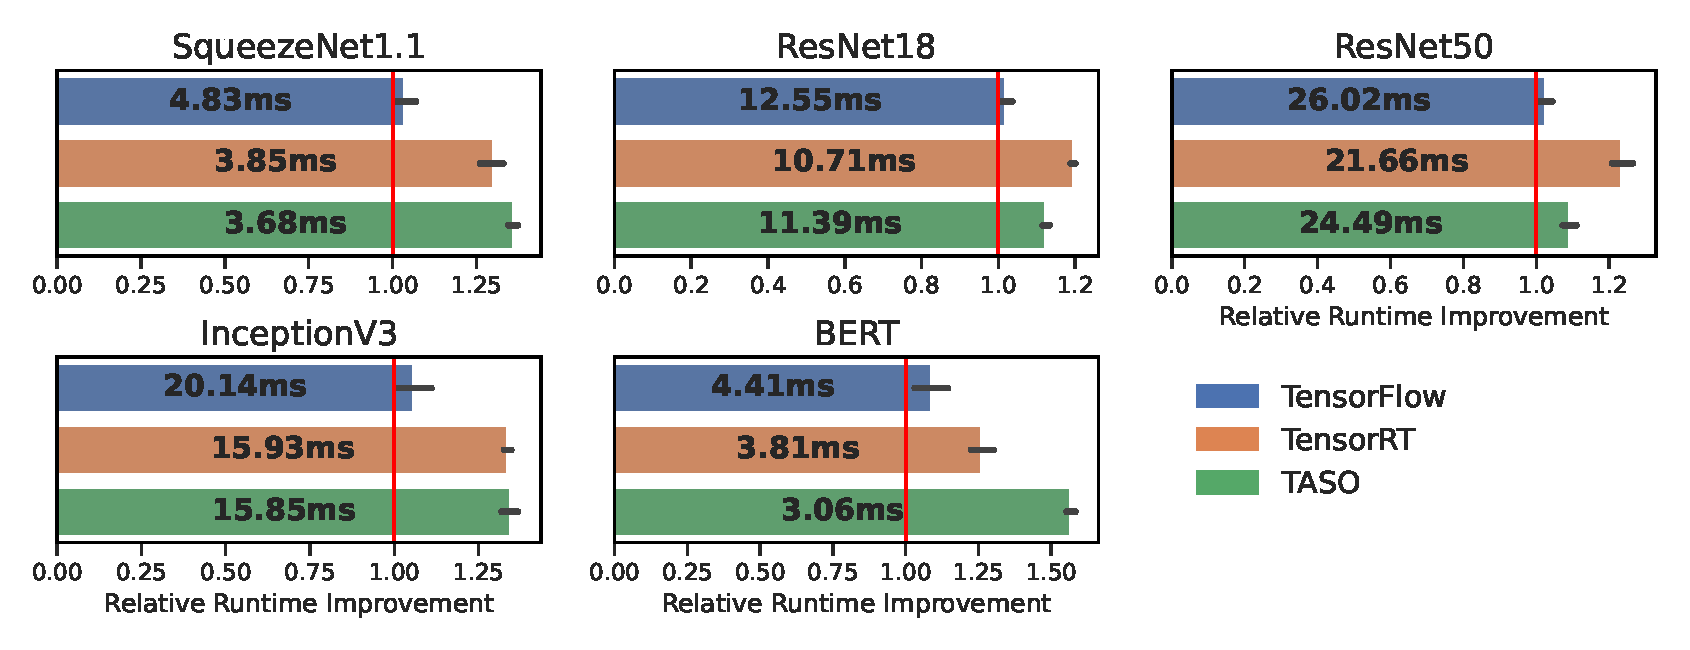
\includegraphics[width=1\columnwidth]{sections/5evaluation/images/runtimes_baseline_h}
  \caption[Baseline runtimes of optimised graphs]{Runtime of optimised graphs using the three baseline optimisation methods. The x-axis shows the relative runtime improvement, a higher relative runtime is better.}
  \label{fig:eval:baseline-runtimes}
\end{figure}

Figure \ref{fig:eval:baseline-runtimes} shows the runtime of each optimised graph described in section \ref{sec:eval:subsec:graphsused} using the three baseline methods, TensorFlow \cite{tensorflow2015-whitepaper}, TensorRT \cite{tensorrt2017} and TASO \cite{jia2019taso}. We observe that TASO outperforms TensorFlow Grappler and TensorRT on BERT by 50.5\% and 43.6\% respectively. On the other hand, with convolutional networks, the optimised graph discovered by TASO has a runtime within $\pm 6$\% compared to TensorRT. Furthermore, we note that during our reproduction of the results found by Jia et al. \cite{jia2019taso}, we used the same value of $\alpha = 1.05$ and a search budget of 50,000 steps. TASO often found the optimal graph within $\sim$5000 steps and the remaining computation steps failed to further improve the estimated runtime.

\begin{figure}[h]
  \centering
  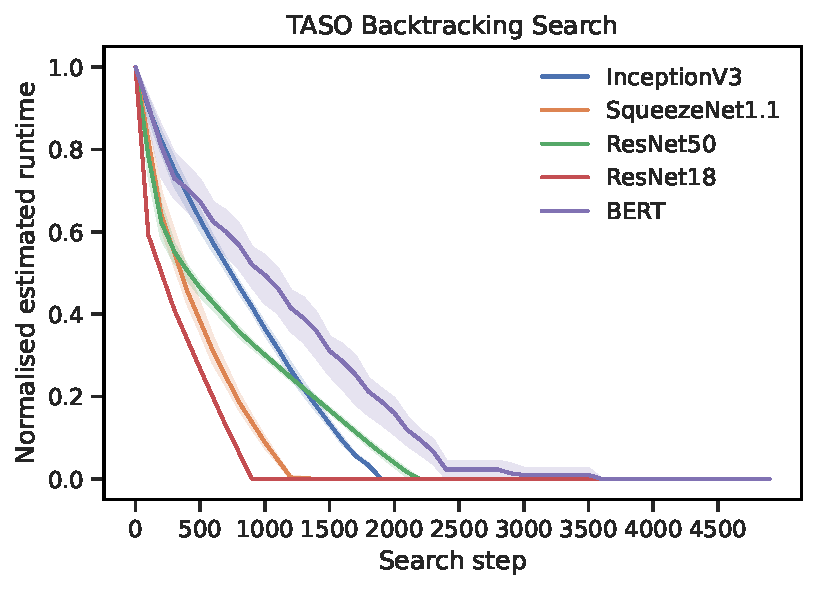
\includegraphics[width=1\columnwidth]{sections/5evaluation/images/taso_graph_search}
  \caption[TASO backtracking search]{We show the estimated runtime improvement, normalised between the minimum and maximum obtained runtimes, for each tested graph. We performed each experiment five times and show the 95\% confidence interval for each graph. We also note that we clipped the plot as after 5000 steps, there was no increase in performance for the remaining 45000 search steps.}
  \label{fig:eval:baseline-taso-search}
\end{figure}

Figure \ref{fig:eval:baseline-taso-search} shows a plot of the runtime estimated by TASO at each step in the search. We repeated each experiment five times and show the confidence interval for each graph. Based upon the results, we observe that TASO did not just take the longest to discover the optimised graph, the variance between runs was the highest compared to other graphs. One reason for this disparity is that it has a vastly different architecture; BERT is a transformer network which, compared to convolution networks, has a greater breadth than depth. As such, when TASO performs the backtracking search, there are far more initial locations in the graph where a substitution can be applied.

\subsection{Model-Free Agent}
\label{sec:eval:subsec:mfagent}

In this section we describe our experiments performed using the model-free agent which acts inside the real environment. Firstly, we trained the agent on each graph under consideration and evaluated its optimised runtime, the results of which we present in figure \ref{fig:eval:mf-agent-runtimes}. In the worst case, the model-free agent performs a series of optimisations that increases runtime by 9\% compared to those discovered by TASO.

\begin{figure}[h]
  \centering
  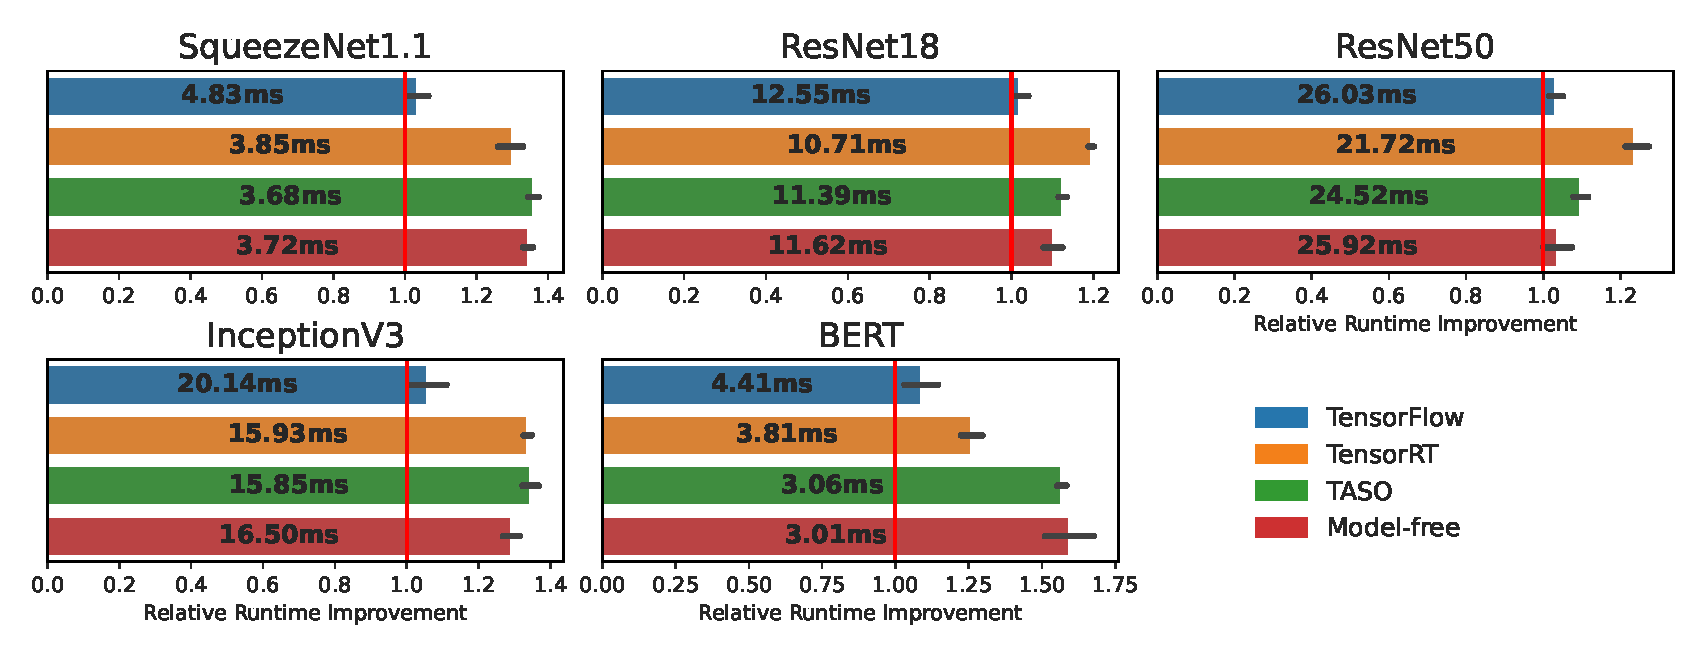
\includegraphics[width=1\columnwidth]{sections/5evaluation/images/runtimes_mf_h}
  \caption[Runtimes of optimised graphs using MF-RL]{Runtime of optimised graphs using an agent trained using the model-free PPO algorithm. We also show the baseline results as comparison. The x-axis shows the relative runtime improvement, a higher relative runtime is better.}
  \label{fig:eval:mf-agent-runtimes}
\end{figure}

\begin{figure}[h]
  \centering
  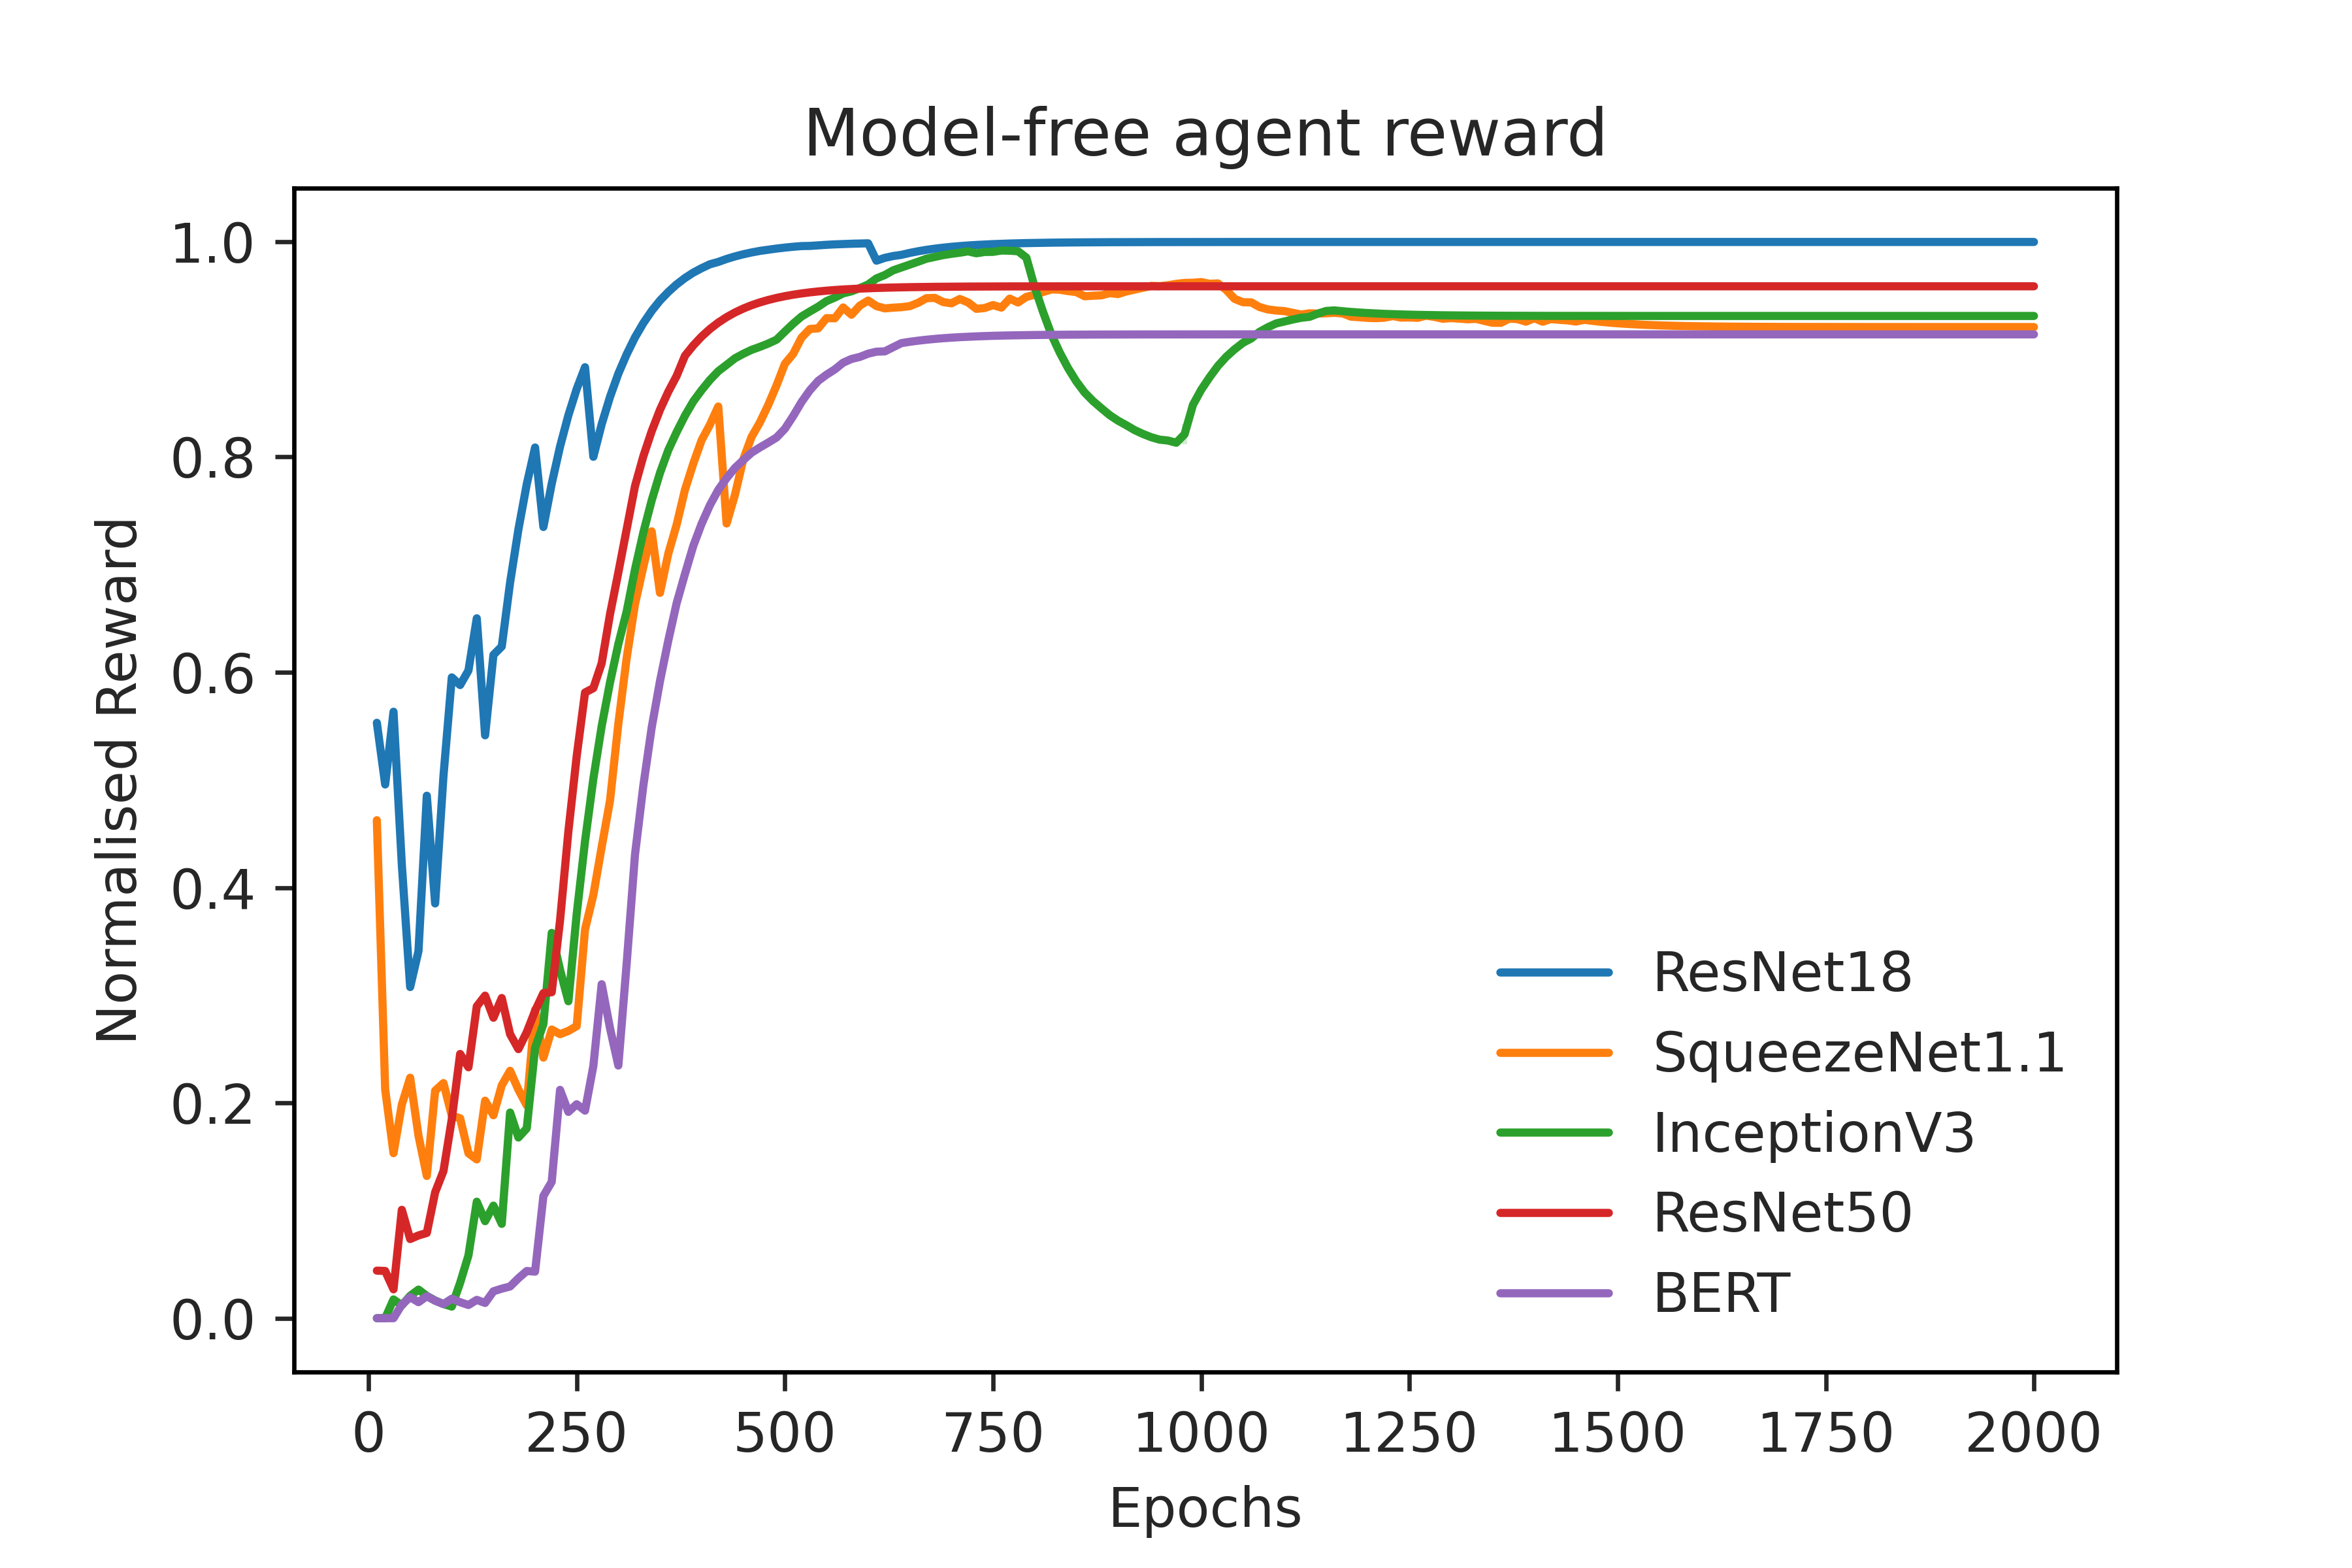
\includegraphics[width=1\columnwidth]{sections/5evaluation/images/mf_training_reward}
  \caption[Epoch reward during training of model-free agent]{Normalised reward of model-free agent produced by the real environment in response to selected actions by the agent}
  \label{fig:eval:mf-agent-reward}
\end{figure}

Figure \ref{fig:eval:mf-agent-reward} shows the reward produced by the model-free agent acting inside the real environment for each graph. Due to the difference in estimated runtime between graphs, we used min-max normalisation to scale the rewards into the same range. First and foremost, it is evident that the graph optimisation using the model-free agent reward converge quickly after only $\sim$1000 epochs with low variation in the average epoch rewards after convergence.

\subsubsection{Reward functions}
\label{sec:eval:subsec:mf:subsubsec:rwd-func}

As we described in section \ref{sec:prob:subsec:rwd}, the design of the reward function used in the training of RL agents is a pivotal part of the agents architecture. In this section, we analyse our proposed reward functions and the effect on the convergence as well as final performance of the trained agents.

\begin{figure}[htbp]
  \centering
  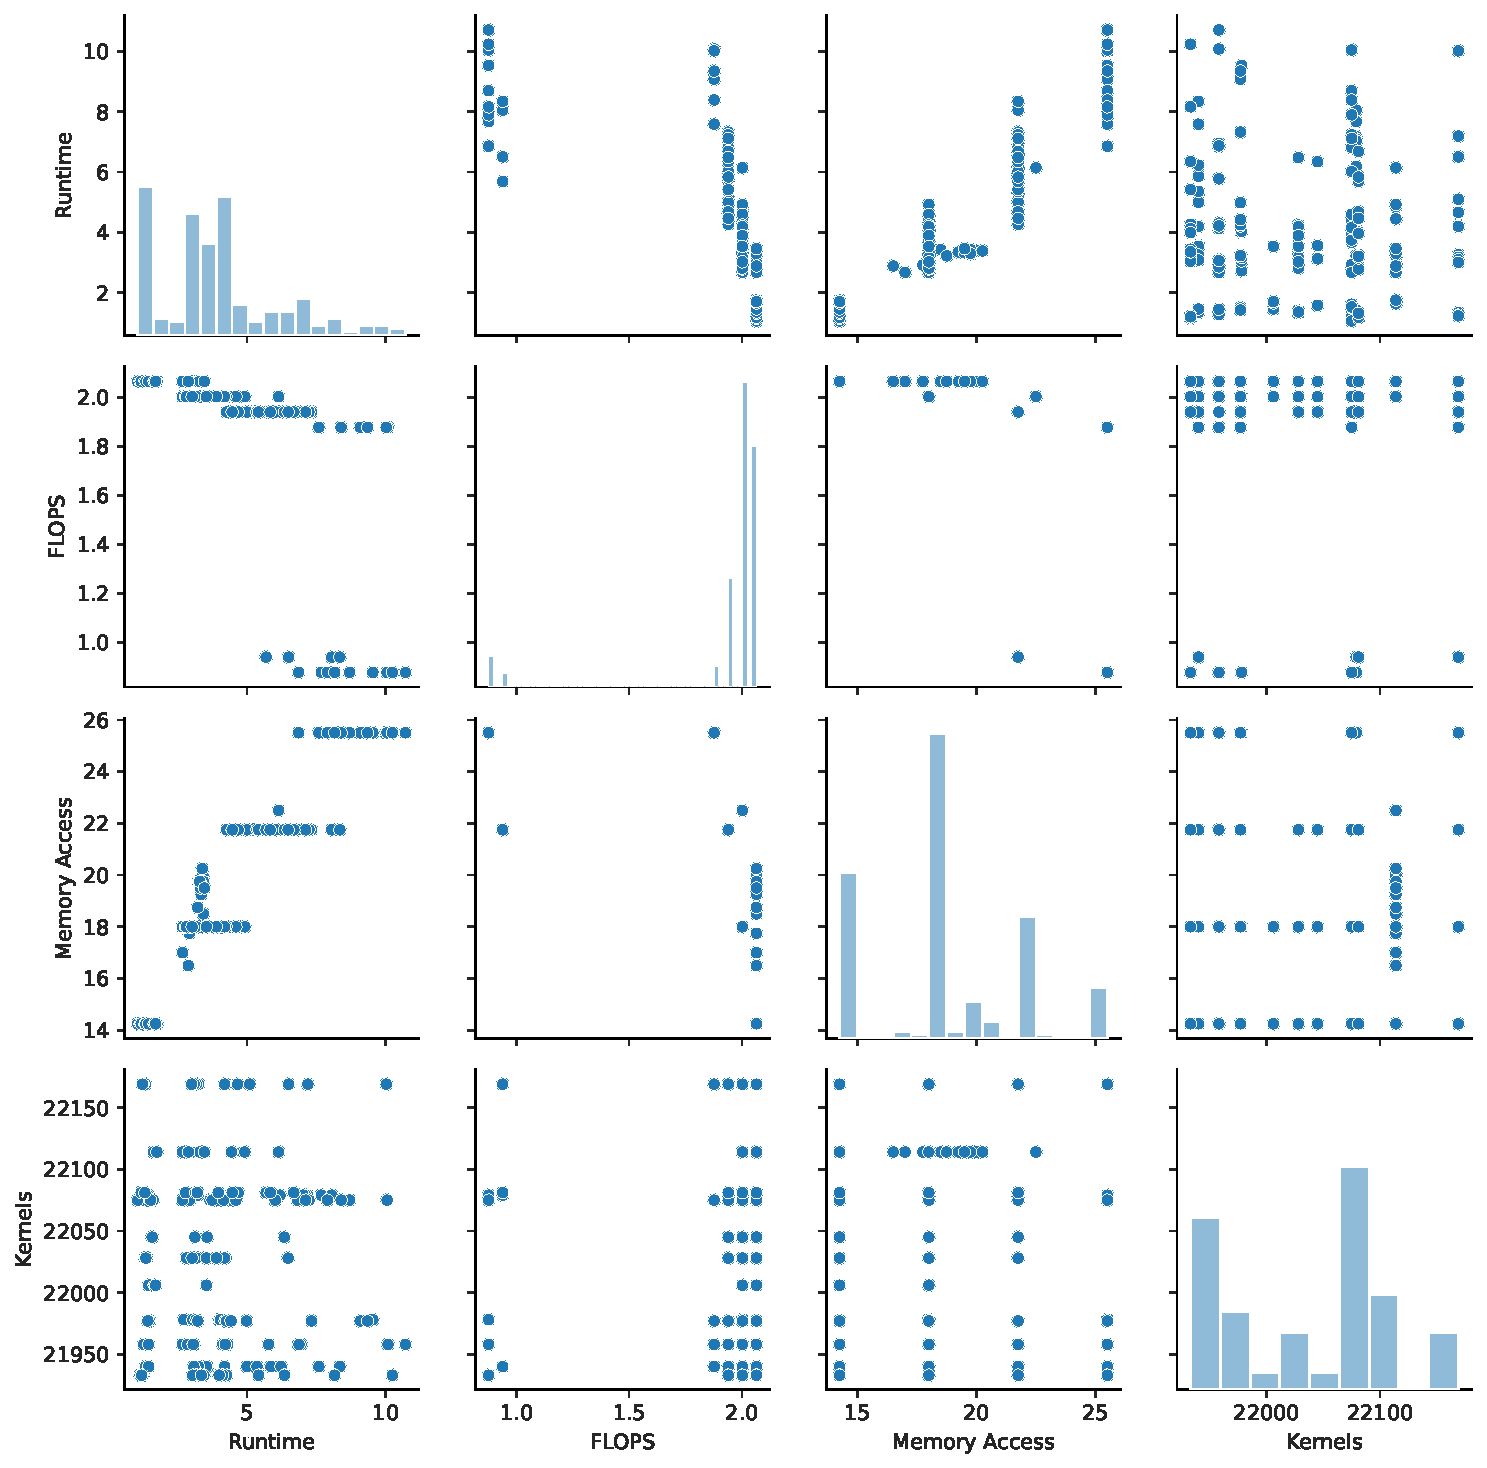
\includegraphics[width=1\columnwidth]{sections/5evaluation/images/pairplot_bert.pdf}
  \caption[Pairwise plot of correlation between runtime metrics]{We show the pairwise correlation between the detailed runtime metrics recorded directly from the TASO environment while training on the BERT graph. We note the strong correlation between the number of memory accesses and estimated runtime improvement.}
  \label{fig:eval:pairplot-bert}
\end{figure}

Figure \ref{fig:eval:pairplot-bert} shows the pairwise relationship between the four detailed runtime measurements which we record at each step of the training process for the BERT graph. We collected the runtime, FLOPS, memory access and number of kernel launches and show the relationship between the values. We note that the estimated runtime and memory accesses have a strong correlation; when the memory access decreases, we see a notable decrease in estimated runtime. 

\begin{figure}[h]
  \centering
  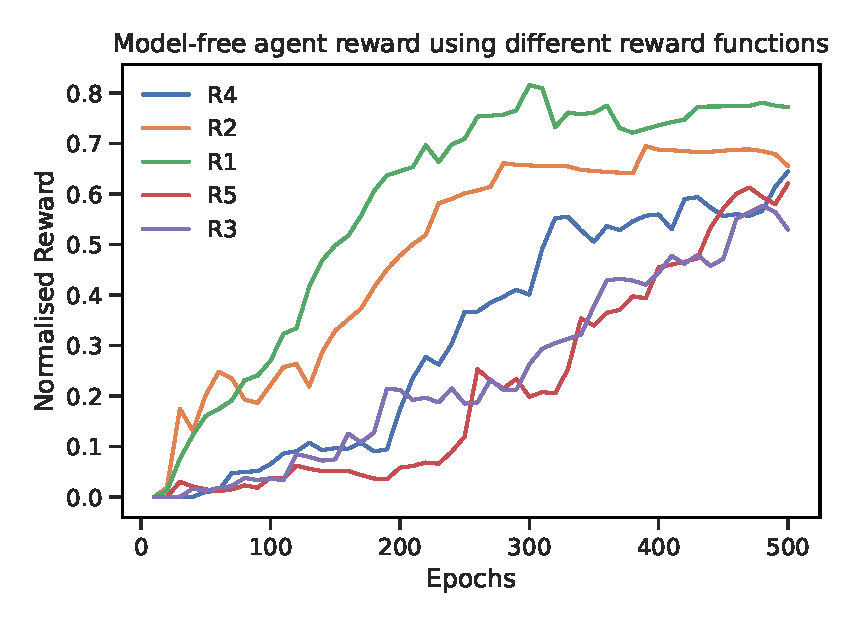
\includegraphics[width=1\columnwidth]{sections/5evaluation/images/mf_reward_func.eps}
  \caption[Agent reward using various reward functions]{We show the normalised reward of each agent using various reward functions while being trained for 500 epochs. R1 uses the second reward function with tuned parameters, R2 uses new runtime reward, R3 uses $\alpha=0.1, \beta=0.9$, R4 uses $\alpha=0.5, \beta=0.5$ and finally, R5 uses incremental runtime improvement.}
  \label{fig:eval:mf-reward-funcs}
\end{figure}

Figure \ref{fig:eval:mf-reward-funcs} shows the effect on convergence of model-free RL agents while training on the BERT graph using various reward functions. Significantly, using a standard, yet naive approach of the first reward function described in section \ref{sec:prob:subsec:rwd} shows that the model-free agent improves at a linear rate as shown by R4 in figure \ref{fig:eval:mf-reward-funcs}. Whereas, using the second reward function and tuned hyperparameters of $\alpha$ and $\beta$, shown by R1, converges the fastest.

However, the rate of convergence does not show the whole picture of the agents performance. We note that the highest performing agent, after the restricted 500 epoch training time, was R1 with an average runtime improvement of $48.7 \pm 3.2\%$. Surprisingly, the second highest performing agent was the agent using R4, the simplest reward function from the set tested, with a performance of $43.2 \pm 2.3\%$.

In order to find the values of hyperparameters $\alpha$ and $\beta$ which results in the agent with the maximum performance, we performed a grid search for $\alpha$ and $\beta = 1 - \alpha$ between the values of $[0, 1]$; we searched between the bounds in increments of $0.1$. After training each agent for 500 epochs and evaluate the performance of each agent three times, we found that the reward function resulting in the highest performance was using the values $0.8$ and $0.2$ for $\alpha$ and $\beta$ respectively.

\subsection{Model-based Agent}
\label{sec:eval:subsec:mbagent}

In this section we first present the results for training an agent inside a world model for each graph individually. Secondly, we compare the model-based agent performance to baseline measurements as well as showing the change in memory usage which is a by product from the applying graph transformations in order to reduce runtime. Furthermore, we also discuss the impact of hyperparameter selection on the agent performance as well as showing the accuracy of the world model in regards to graph reward prediction.

\subsubsection{Runtime Performance}
\label{sec:eval:subsec:mb:sec:runtimeperf}

Figure \ref{fig:eval:world-model-runtimes} shows the runtime of the optimised graphs for the model-based agents trained inside the fully hallucinogenic world model. Each agent was trained inside a world model using rollouts from its respective graph as described in section \ref{sec:rlopt:subsec:actionctrl}. We trained the agents for a maximum of 1000 epochs, in mini-batches of 10 epochs. Additionally, we used a fixed learning rate for both the policy and value networks during training of the controller agent network.

\begin{figure}[h]
  \centering
  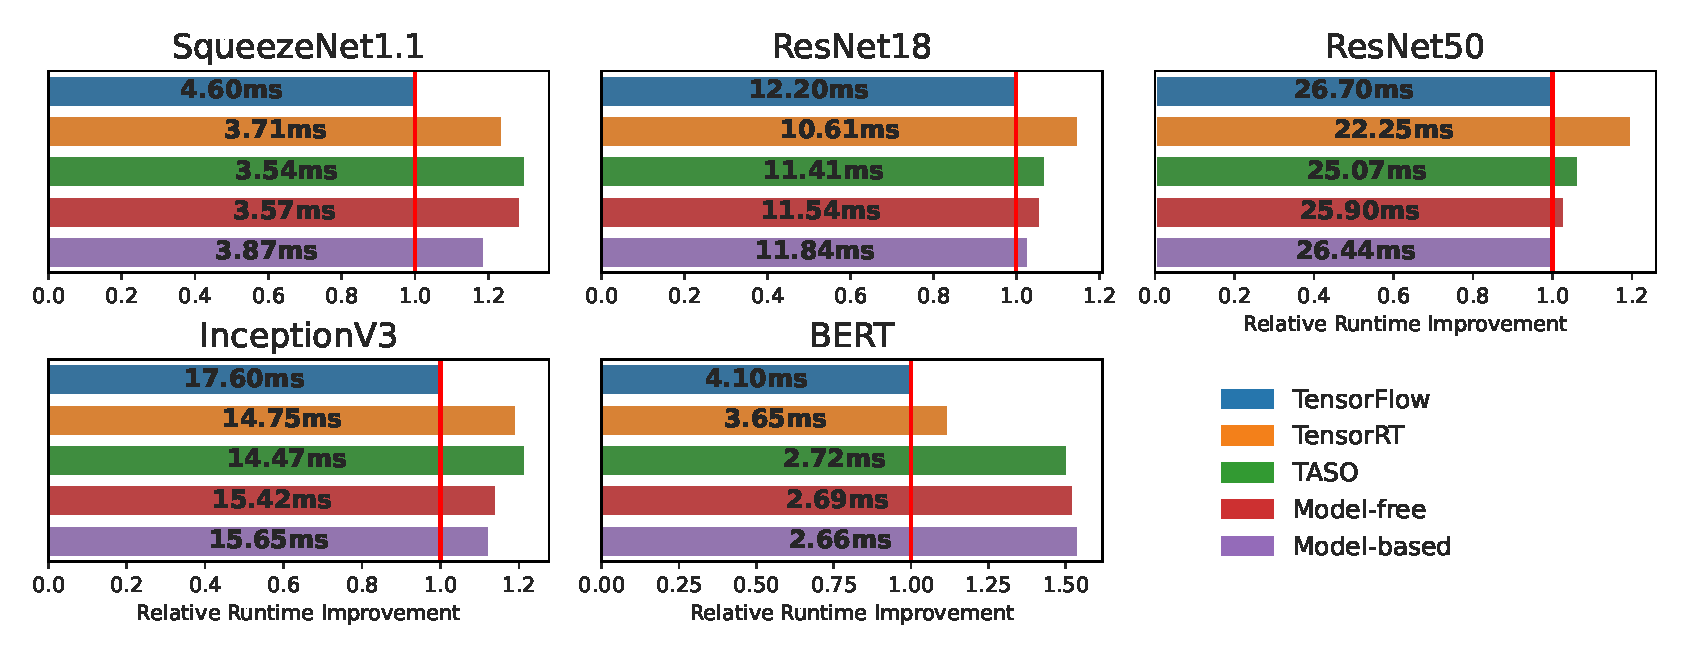
\includegraphics[width=1\columnwidth]{sections/5evaluation/images/runtimes_all_h}
  \caption[Runtimes of optimised graphs using a model-based controller]{Runtime of optimised graphs using an agent trained using the model-based world model. We also show the baseline results as comparison. The x-axis shows the relative runtime improvement, a higher relative runtime is better.}
  \label{fig:eval:world-model-runtimes}
\end{figure}

Firstly, we note that training the agents on convolutional networks, especially SqueezeNet1.1 and InceptionV3, the model-based agent failed to outperform TASO, we still decreased the runtime compared to the baseline graph produced by TensorFlow Grapper. Importantly, we observe that the model-based agent outperformed all baseline approaches on the BERT transformer network; we improved the runtime by 54.1\% and 7.3\% compared to TensorFlow and TASO respectively. Figure \ref{fig:eval:xfer-heatmap} shows the transformations applied by the model-based agent on the test graphs and compared to TASO, we only apply a single transformation over 20 times---compared to TASO which uses four distinct transformations produce the optimised graph.

% [TODO - describe the type of transformations applied to better compare]

Compared to the strictly model-free agent that was trained in the real environment, our model-based agent achieved a similar level of performance in the majority of the tested graphs. The model-free agent was trained for 2000 epochs and, by extension, over 4,000,000 interactions with the real environment. Comparatively, the model-based agent performed approximately 1,000,000 interactions with the real environment as the agent did not interact with the real environment while training inside the world model. Therefore, it is evident that by training inside the world model we improved the sample efficiency of the agent. On the other hand, the performance of the agent decreased compared to the model-free agent in four of the five tested graphs.

Furthermore, an important consideration when training inside a systems environment is the wall-clock time for stepping the environment to a new state based upon the agent action. We analysed the time required to perform a single step while training the ResNet50 graph. We found that stepping the world model (performing inference of the world-model) takes, on average, 10ms whereas stepping the real environment takes on average 850ms. Thus, although the performance of the model-based agent was comparatively lower, our wall-clock time for required for training was reduced by a factor of 85x.

\subsubsection{Memory Usage}

% Table of memory usage
\begin{table}[htbp]
  \centering
  \resizebox{\columnwidth}{!}{
    \begin{tabular}{@{}ccccc@{}}
      \toprule
      \multicolumn{1}{l}{} & \multicolumn{2}{c}{Baseline (TF)}                                         & \multicolumn{2}{c}{Optimised (MB-RL)} \\ \midrule
      \multicolumn{1}{l}{} & \multicolumn{1}{l}{Inf. time (ms)} & \multicolumn{1}{l}{Mem. usage (GiB)} & \multicolumn{2}{c}{\% Improvement}    \\
      ResNet18      & 12.2 & 1.18 & 3.0\%  & 1.1\% \\
      ResNet50      & 26.7 & 2.34 & 1.0\%  & 0.6\% \\
      InceptionV3   & 17.6 & 2.11 & 12.5\% & 2.3\% \\
      SqueezeNet1.1 & 4.6  & 1.14 & 18.9\% & 1.8\% \\
      BERT          & 4.1  & 0.26 & 54.1\% & 4.5\% \\ \bottomrule
      \end{tabular}
  }
  \caption[Memory usage of optimised graphs]{Relative performance improvement of the graphs optimised by the model-based agent. We show the inference time, and memory used for performing inference on the model.}
  \label{table:eval:graph-mem-usage}
\end{table}

Table \ref{table:eval:graph-mem-usage} shows the percentage improvement of both the inference time and the memory used for performing inference on the optimised models. Importantly, although we tasked the agent to optimise for reducing the runtime of the graphs, we observe an unintended secondary effect of a reduction in memory usage of up to 4.5\% over the baseline TensorFlow model.

\subsubsection{World-model accuracy}
\label{sec:eval:subsubsec:wm-acc}

\begin{figure}[h]
  \centering
  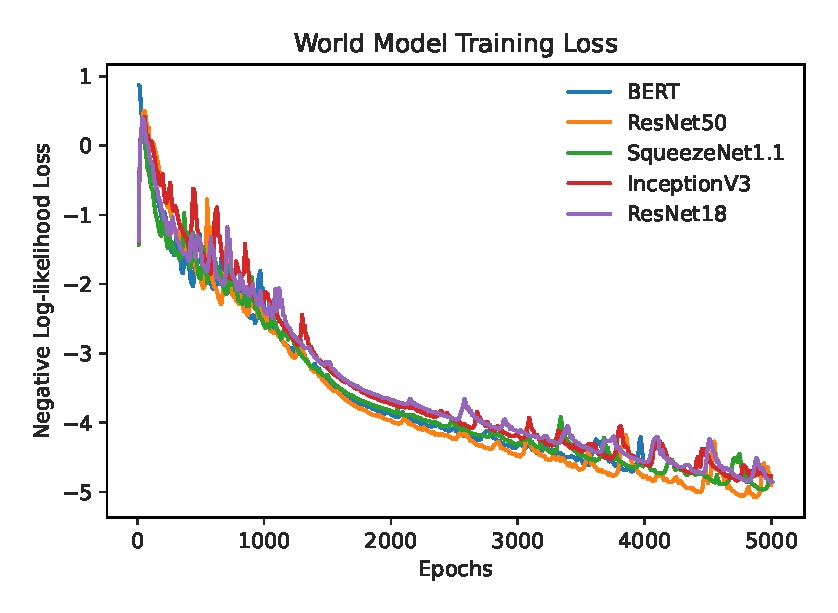
\includegraphics[width=1\columnwidth]{sections/5evaluation/images/mb_training_loss}
  \caption[Log-likelihood loss of world models]{Training plot of the log-likelihood loss for our world model on the five test graphs.}
  \label{fig:eval:world-model-loss}
\end{figure}

The training of the model-based agent is split into two parts. First, we train the world-model, the network that learn to simulate the environment dynamics, and secondly, we train the controller network inside the world-model. In this section, we show the convergence of the world model during training in figure \ref{fig:eval:world-model-loss}. The figure is a plot of the log-likelihood loss per training epoch for each graph. We used the same hyperparameters for training each world model as well as decaying the learning rate over the course of 2000 epochs with a 2nd-degree polynomial decay policy. The MDN-RNN is trained with 8 Gaussians and 256 hidden units, all other hyperparameters used in training the MDN-RNN world model are the same as those used by Ha and Schmidhuber \cite{ha2018worldmodels}, unless otherwise stated.

% TODO explain more!

\begin{figure}[h]
  \centering
  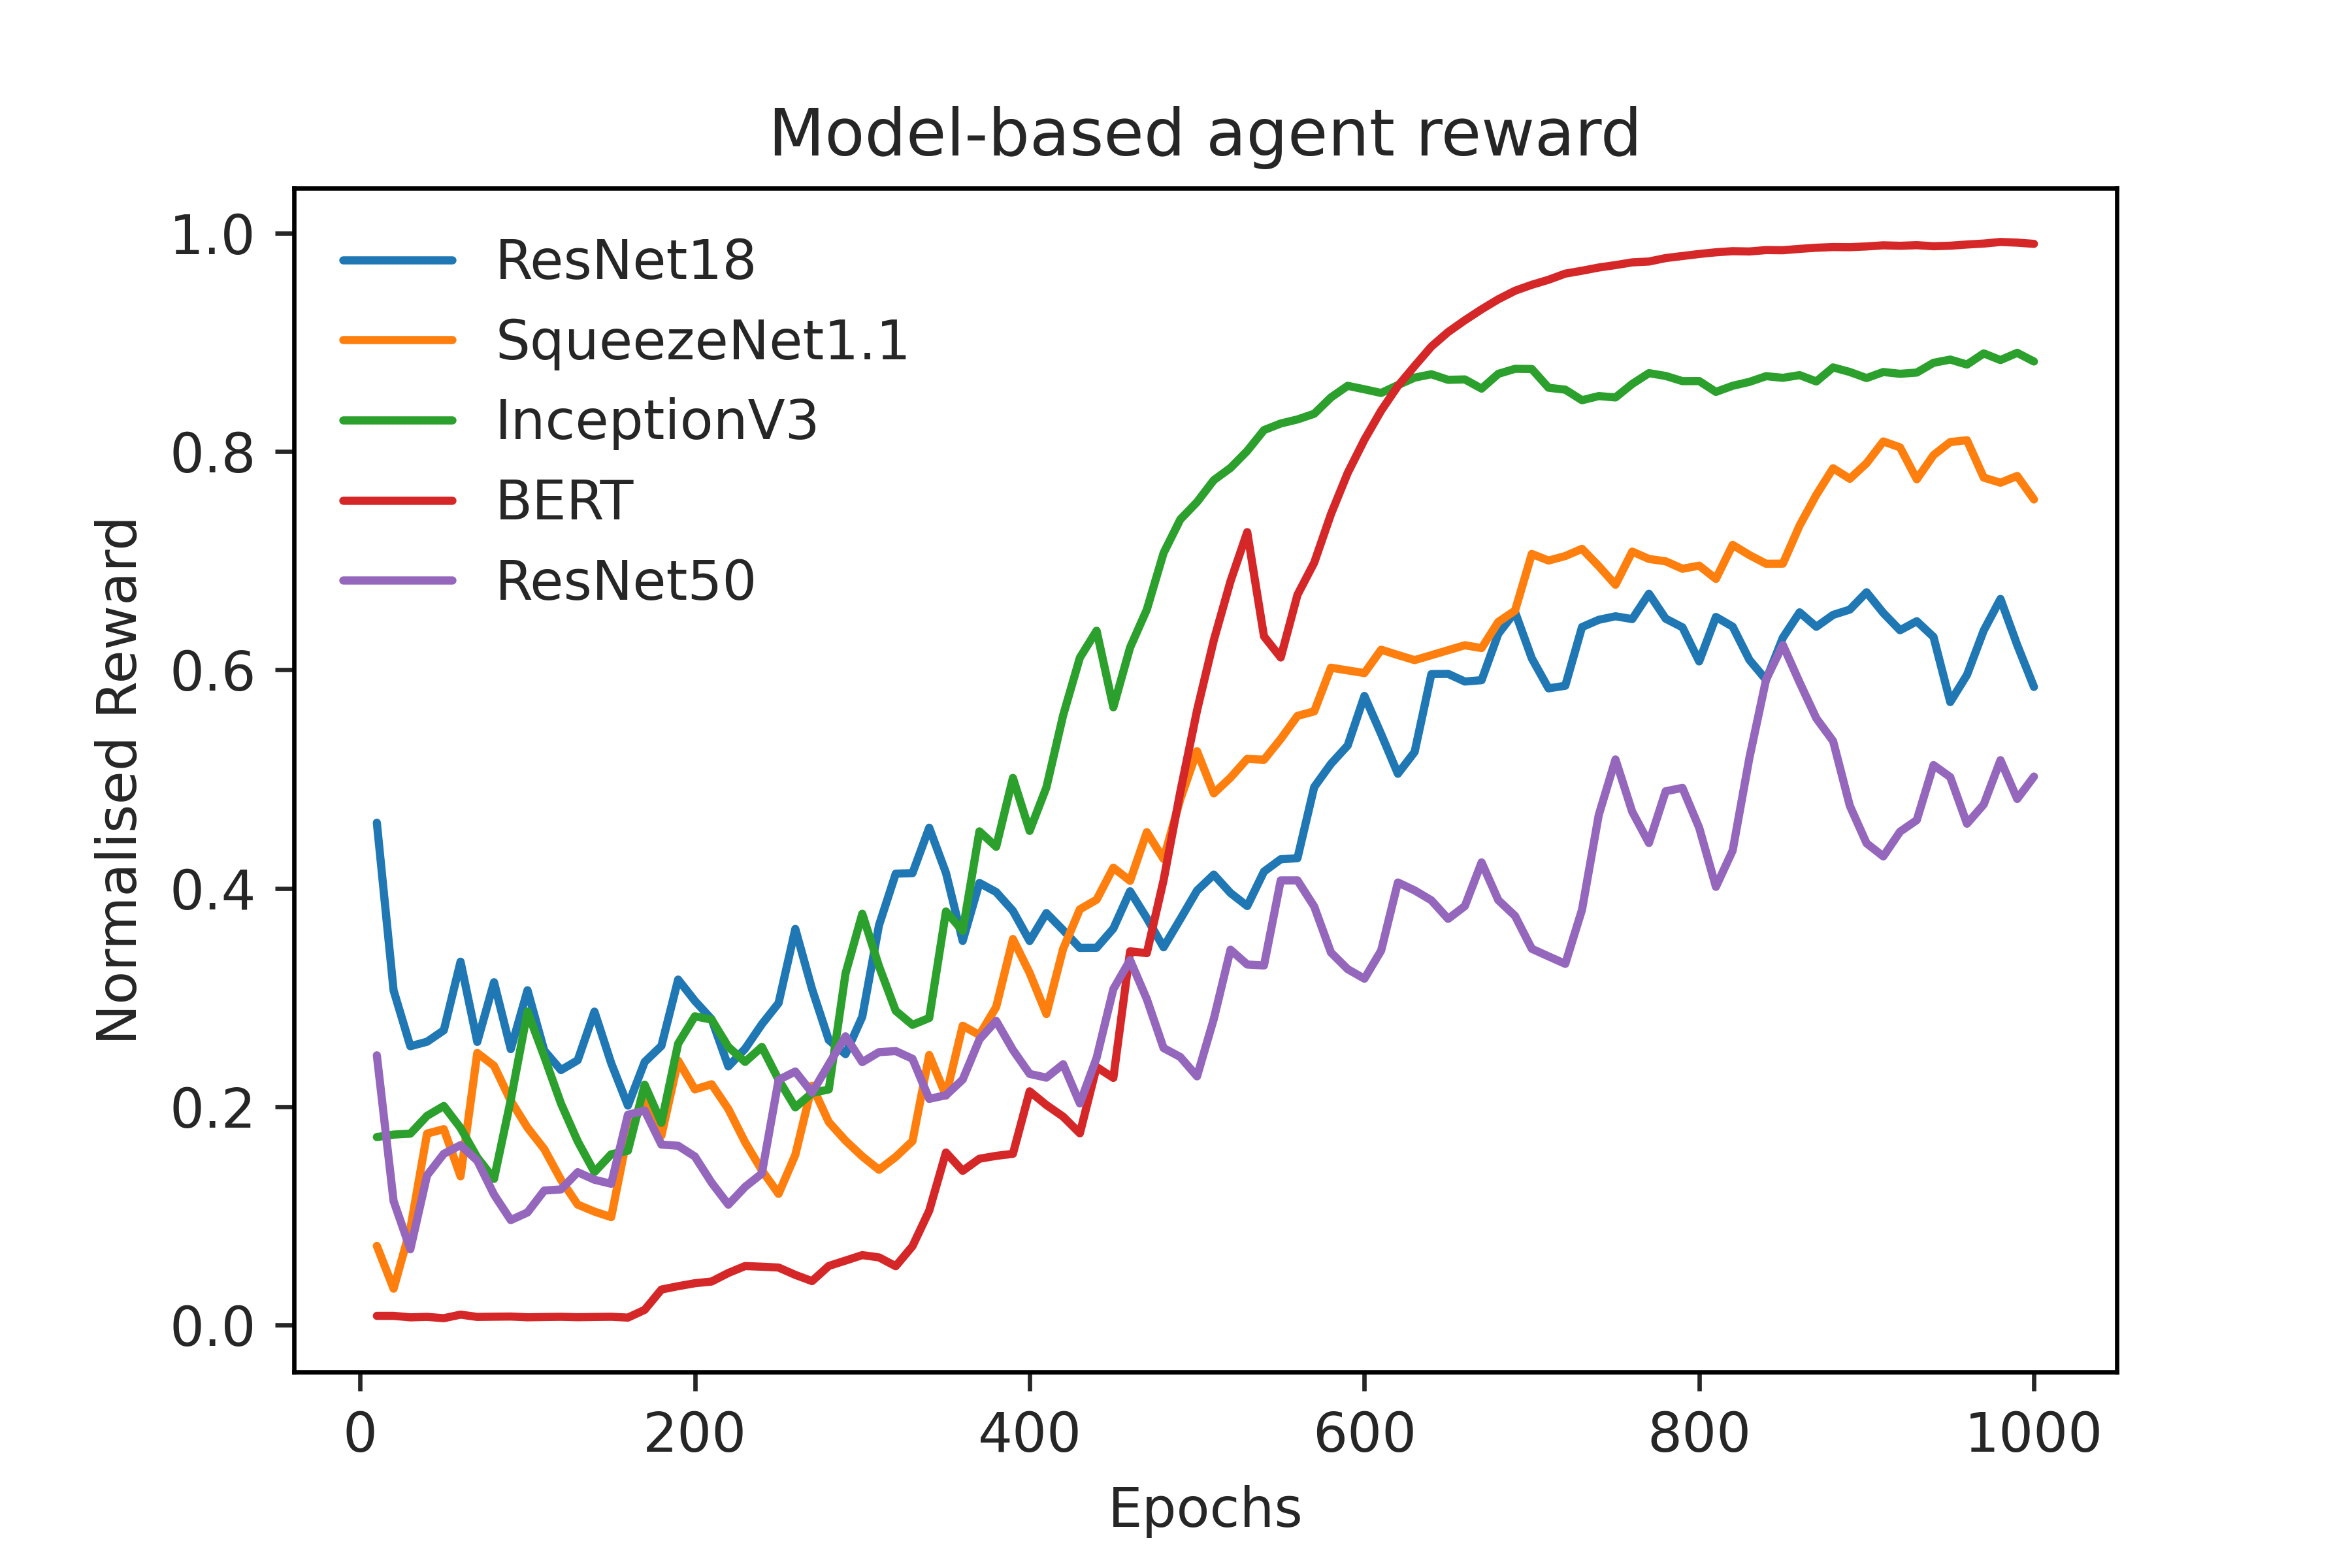
\includegraphics[width=1\columnwidth]{sections/5evaluation/images/mb_ctrl_training_reward}
  \caption[Predicted epoch reward during training of agent in world model]{Predicted reward produced by the world model while training the agent inside a the imagined environment. All rewards are normalised into the same range.}
  \label{fig:eval:world-model-pred-reward}
\end{figure}

Figure \ref{fig:eval:world-model-pred-reward} shows the reward (decrease in estimated runtime) for each graph as predicted by the world model during training. As the tested graphs have a wide range of epoch rewards, we perform min-max normalisation to scale the plots into the same range. We observe the same results as figure \ref{fig:eval:world-model-runtimes} in which the optimisations applied to BERT during training results in the optimal graph found after 700 epochs. On the other hand, graphs such as ResNet 18/50 are less stable during training with a high epoch to epoch variation in rewards. In comparison to the rewards received by the model-free agent during training, we note that the strictly model-free agent was more stable during training, and additionally, consistently found the optimised graph after approximately 1000 epochs.

\subsubsection{Discussion}

If we assume that both the model-free and model-based agents should achieve a similar level in performance once trained, the results in figure \ref{fig:eval:world-model-pred-reward} and \ref{fig:eval:mf-agent-reward} show that the agents trained in the world model are less stable with a higher reward variance. We hypothesise that there are three factors for such a discrepancy to occur:

\begin{itemize}
  \item Imperfect world-model reward predictions leading to incorrect (or invalid) actions being performed
  \item Next state prediction by the world-model generating states that are invalid due to poor generalisation of the model
  \item Incorrect action mask predictions that would lead to a divergence in between the world-model state and real environment state 
\end{itemize}

In an attempt to resolve the issues highlighted above, we performed further experiments which we believe would aid in both reducing the variance in reward prediction as well as stabilise the world-model during training to prevent state divergence over time. We performed a temperature sweep of the hyperparameter $\tau$ which is used in training agent inside the world model, shown in section \ref{sec:eval:subsec:temp-sweep}.

% Secondly, we also investigated splitting the prediction components of the world model such that we do not predict the next state, rewards, terminals and masks in a single model. Rather, we use a separate network to perform reward prediction using the hidden state, $h_t$ from the MDN-RNN as well as the latent graph state $s_t$.

% [TODO finish]


\subsubsection{Temperature Sweep}
\label{sec:eval:subsec:temp-sweep}

\begin{table}[htbp]
  \centering
  \begin{tabular}{@{}lll@{}}
  \toprule
  Temperature  & World-model Score        & Real Score                \\ \midrule
  0.1          & -6.67\% $\pm$ 0.6\%          & -43.92\% $\pm$ 5.1\%         \\
  0.5          & -7.75\% $\pm$ 0.3\%          & -55.33\% $\pm$ 6.7\%         \\
  0.75         & -9.10\% $\pm$ 0.4\%          & -55.80\% $\pm$ 5.2\%         \\
  1.0          & -8.85\% $\pm$ 1.2\%          & -55.78 $\pm$ 4.0\%           \\
  1.2          & -9.91\% $\pm$ 0.8\%          & -57.01\% $\pm$ 3.9\%         \\
  \textbf{1.5} & \textbf{-8.37\% $\mathbf{\pm}$ 0.6\%} & \textbf{-58.23\% $\mathbf{\pm}$ 3.6\%} \\
  1.75         & -9.92\% $\pm$ 1.0\%          & -52.07\% $\pm$ 5.8\%         \\
  2.0          & -9.65\% $\pm$ 0.8\%          & -46.12\% $\pm$ 5.4\%         \\
  2.5          & -10.04\% $\pm$ 2.0\%         & -41.14\% $\pm$ 10.2\%         \\
  3.0          & -10.38\% $\pm$ 1.9\%         & -51.32\% $\pm$ 7.2\%         \\ \bottomrule
  \end{tabular}
  \caption[Rewards using range of temperatures]{Temperature sweep of trained model-based agent optimising the BERT network. We ran each experiment five times and show both the average performance improvement as well as the variance between runs.}
  \label{table:eval:agent-temperatures}
\end{table}

Table \ref{table:eval:agent-temperatures} shows the results from performing a temperature sweep in which we used different values of $\tau$ while training the agent in a world model. After training, we evaluated the agent which produced an optimised graph that we evaluated to determine average runtime. The table shows the average reduction in runtime and standard deviation, averaged over five runs, compared to the unoptimised graph. The motivation for using a range of temperatures is that a higher value of $\tau$ leads to softer targets for the agent to predict, thereby improving generalisation. Conversely, a lower value of $\tau$ presents hard targets and thus when $\tau = 1.0$, it is equivalent to using the unmodified mixing weight, $\pi$, of the MDN.

Based upon the results in table \ref{table:eval:agent-temperatures} from the conducted experiments, we note that the world model agents are stable to temperatures within the range of $\tau = 0.5$ to $\tau = 1.75$. Although the runtime improvement world-model from the environment is consistently above 6\%, we observe a large difference between the predicted runtime improvement and the real environment reward.

% Despite the experiments performed in section [TODO] \ref{sec:eval:subsubsec:wm-acc} which shows a low MSE between the predicted and real scores, during evaluation we see a large divergence between the two scores. Therefore, we performed further experiments to evaluate the performance of the agents inside the world-model using a composite model in which the reward prediction is conducted in a separately trained network.

% [TODO include results from separate reward prediction network]

\subsubsection{Agent Convergence}
\label{sec:eval:subsec:agent-conv}

\begin{figure}[ht]
  \centering
  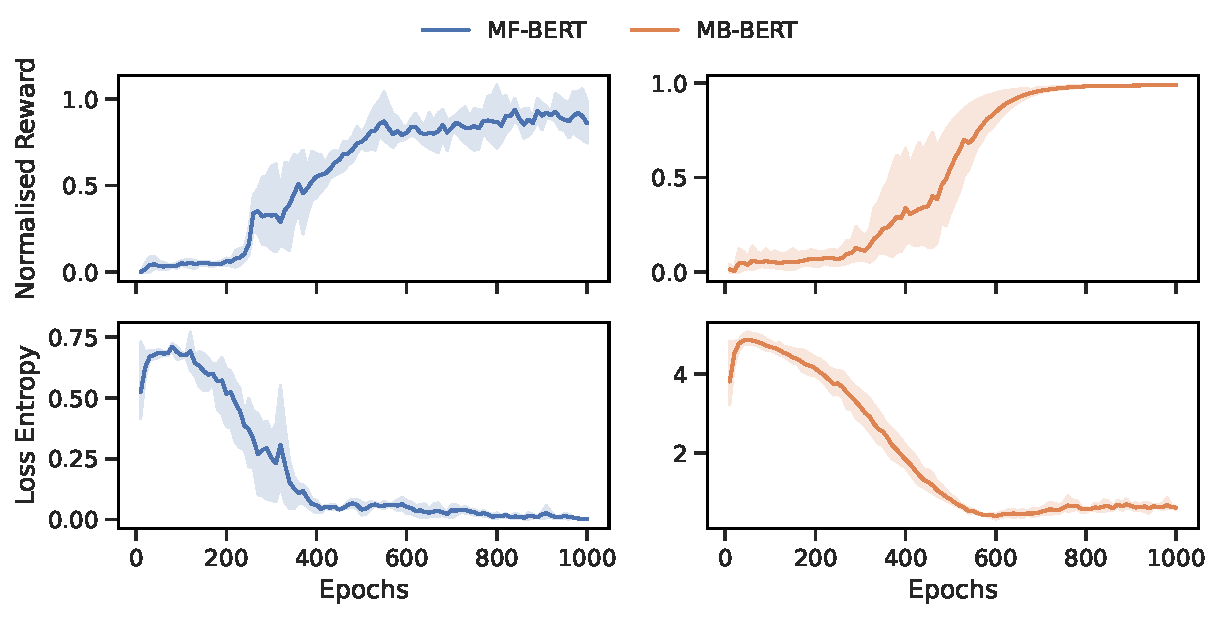
\includegraphics[width=1\columnwidth]{sections/5evaluation/images/agent_convergence.pdf}
  \caption[Convergence line plots of MF and MB approaches]{Agent reward and loss for model-free and model-based agents shown on the left (blue) and right (orange) respectively. We trained the agents on the BERT graph for 1000 epochs and repeated the experiments five times. We show the 95\% confidence interval in the shaded area of each plot.}
  \label{fig:eval:agent-mf-mb-convg}
\end{figure}

As we have previously claimed, there are many benefits to using a world model as the environment where we train the controller agent. In Figure \ref{fig:eval:agent-mf-mb-convg} we show the agent reward and loss during training for 1000 epochs on the BERT graph using model-free (MF) and model-based (MB) agents. Also, we used the results from our previous temperature sweep experiment by choosing the temperature $\tau = 1.5$ for use when training the controller. We found that the model-based agent, when trained using tuned hyperparameters, was more stable than the MF agent trained inside the real environment; the variance between runs was lower for the model-based agent compared to the MF agent. However, we found that the variance in the optimised runtime of the models produced by the MF agent was larger than the MB agent, with a variance of $6.1\%$ and $3.6\%$ respectively.


\subsubsection{Graph transformations}

\begin{figure}[ht]
  \centering
  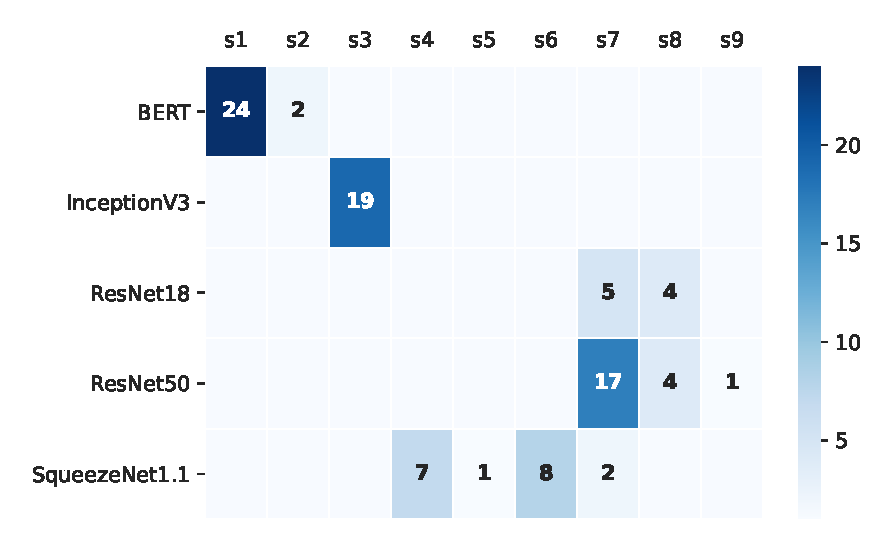
\includegraphics[width=1\columnwidth]{sections/5evaluation/images/xfer_heatmap}
  \caption[Heatmap of graph transformations applied by MB controller]{Heatmap showing the transformations applied by the trained controller acting inside the world model. Although there are over 100 possible transformations, we only show the transformations applied onto at least one graph. The counts for each transformation show the number of times it has been applied.}
  \label{fig:eval:xfer-heatmap}
\end{figure}

Figure \ref{fig:eval:xfer-heatmap} shows a heatmap of the various graph transformations which have been applied by a trained model-free agent during evaluation. Notably, the optimisations applied to the ResNet18/50 graphs apply similar transformations, those targeting the convolutions in the network; as the networks are composed of alike convolutional operators, with different depths, we apply analogous transformations. On the otherhand, for recurrent networks such as BERT, we only apply relatively few transformations. This is in stark contrast to the series of transformations found by TASO which applies four distinct substitutions in comparison to the two applied by our approach. Despite the large disparity in both the specific transformations as well as number of times we applied transformations, the performance difference between TASO and our proposed method is small.

\section{Discussion}
Throughout this chapter we have evaluated our claims which we formed in the introduction. We have provided the results to various experiments covering the reinforcement of our baseline measurements and those which show the performance of the proposed agents. Overall, we have found that our proposed approach outperforms the TensorFlow optimisation strategy on all graphs. However, in some cases, namely the deeper convolutional networks such as ResNet50 and InceptionV3, our agents failed to apply optimisations that outperform those performed by TensorRT and TASO.

In examining the model-based agent performance, we found that a world-model is able to accurately learn and simulate the transition dynamics of an environment, showing that despite the complex nature of the state-action transitions the world-model is flexible to learn its behaviour and adapt to previously unseen state-action pairs. 

Notably, although the state-action prediction and the terminal state prediction was accurate, we found the reward prediction had a large error when compared to the real reward produced by the environment. However, and surprisingly, this disparity between the two rewards did not have a significant impact on the agent performance as we showed in section \ref{sec:eval:subsec:temp-sweep}, the agent trained inside the world model is stable to a wide range of operating conditions.

Finally, the primary takeaway from these experiments is that reinforcement learning, especially model-based methods, are extremely powerful and can learn to model complex dynamic systems and provide important benefits. Nonetheless, we note that such methods still suffer instability during training, and imperfections in the world-model leads to agent exploitation of the faulty environment and therefore poor performance in the real environment---tuning of the world-model hyperparameters remains vital to producing a stable, performant agent. 
% TODO List:

% - Hyperparameter search

% - Reward prediction for model-based method (Separate reward pred network, compare MSE)

% - Show sample graph xfers graphically


\chapter{Conclusion and Future Work}

\section{Conclusion}

\section{Future Work}

%\appendix
%\singlespacing

\bibliographystyle{unsrt} 
\bibliography{ref} 

\end{document}
